\documentclass[aspectratio=169,11pt]{beamer}

\newcommand{\currentpart}{2}
% ============================================================================
% Quantitative Research -- shared preamble for all five slide decks
%
% Every deck starts with
%     \documentclass[aspectratio=169,11pt]{beamer}
%     % ============================================================================
% Quantitative Research -- shared preamble for all five slide decks
%
% Every deck starts with
%     \documentclass[aspectratio=169,11pt]{beamer}
%     % ============================================================================
% Quantitative Research -- shared preamble for all five slide decks
%
% Every deck starts with
%     \documentclass[aspectratio=169,11pt]{beamer}
%     \input{../common/preamble.tex}
%     \newcommand{\currentpart}{<k>}
% so that layout, colours, boxes and code listings are identical everywhere.
% ============================================================================

% ======================== Packages ========================
\usepackage[utf8]{inputenc}
\usepackage[T1]{fontenc}
\usepackage[english]{babel}
\usepackage{graphicx}
\usepackage{booktabs}
\usepackage{amsmath,amssymb,amsfonts}
\usepackage{mathtools}
\usepackage{xcolor}
\usepackage{colortbl}
\usepackage{array}
\usepackage{multicol}
\usepackage{verbatim}          % provides the comment environment
\usepackage{tikz}
\usepackage{pgfplots}
\pgfplotsset{compat=1.18}
\usetikzlibrary{arrows.meta,positioning,fit,backgrounds,shapes.geometric,calc,decorations.pathreplacing}
\usepackage{listings}
\usepackage{hyperref}
\usepackage{pgfpages}          % notes on a second screen (only if enabled)

% ======================== Speaker notes (talk-tracks) ========================
% The decks compile WITHOUT notes by default. To get a version with the
% talk-tracks, uncomment exactly ONE of the lines below and recompile:
% \setbeameroption{show notes}                          % notes as separate pages
% \setbeameroption{show notes on second screen=right}   % slides left, notes right

% ======================== Math fonts ========================
% Beamer typesets text in sans serif; make \mathrm and \mathbf match it
% (otherwise SE, TP, RSS print in serif and \mathbf falls back to non-bold).
\renewcommand{\bfdefault}{bx}   % CM sans has bold extended (bx) only
\DeclareMathAlphabet{\mathrm}{T1}{cmss}{m}{n}
\DeclareMathAlphabet{\mathbf}{T1}{cmss}{bx}{n}
\SetMathAlphabet{\mathrm}{bold}{T1}{cmss}{bx}{n}
\SetMathAlphabet{\mathbf}{bold}{T1}{cmss}{bx}{n}
\SetSymbolFont{operators}{bold}{OT1}{cmss}{bx}{n}
% Beamer re-declares \mathrm at \begin{document}; re-apply the sans-serif version
\AtBeginDocument{\SetMathAlphabet{\mathrm}{normal}{T1}{cmss}{m}{n}%
                 \SetMathAlphabet{\mathrm}{bold}{T1}{cmss}{bx}{n}}

% ======================== Colour palette (matched to plots / Madrid) ========
\definecolor{hsbiblau}{HTML}{3333B2}
\definecolor{hsbiblaudunkel}{HTML}{1C1C6E}
\definecolor{hsbiorange}{HTML}{E69F00}
\definecolor{hsbigrau}{HTML}{9A9A9A}
\definecolor{hsbirot}{HTML}{C0392B}
\definecolor{hsbigruen}{HTML}{2E8B57}
\definecolor{hsbiviolett}{HTML}{8C3CA0}   % 4th comparison colour (e.g. candidate lines)

% ======================== Theme ========================
\usetheme{Madrid}
\usecolortheme{default}
\setbeamertemplate{navigation symbols}{}
\setbeamertemplate{blocks}[rounded][shadow=false]
\setbeamerfont{section in head/foot}{size=\tiny}

% Horizontal section navigation bar in the headline
\setbeamertemplate{headline}{%
  \leavevmode%
  \hbox{%
    \begin{beamercolorbox}[wd=\paperwidth,ht=2.5ex,dp=1.125ex]{section in head/foot}%
      \scriptsize\insertsectionnavigationhorizontal{\paperwidth}{}{\hskip0pt plus1filll}%
    \end{beamercolorbox}%
  }%
}

% Footline: lecture part, current section (if any) and slide number
\newcommand{\footsection}{%
  \setbox0=\hbox{\insertsection}%
  \ifdim\wd0>0pt\ \textbar\ \insertsection\fi}
\setbeamertemplate{footline}{%
  \leavevmode%
  \hbox{%
  \begin{beamercolorbox}[wd=\paperwidth,ht=2.5ex,dp=1.125ex]{author in head/foot}%
    \hspace*{2em}Part~\currentpart\footsection\hfill\insertframenumber{}/\inserttotalframenumber\hspace*{2em}%
  \end{beamercolorbox}%
  }%
}

% Automatic section overview slide. Decks with many sections define
%   \newcommand{\overviewleft}{1-4}\newcommand{\overviewright}{5-8}
% before \begin{document} to get a two-column overview.
\newcommand{\overviewtoc}[1]{%
  \tableofcontents[currentsection,sectionstyle=show/shaded,
                   subsectionstyle=show/show/hide,sections={#1}]}
\newcommand{\sectionoverview}{%
  \ifdefined\overviewleft
    \begin{columns}[T]
      \column{0.49\textwidth}\overviewtoc{\overviewleft}
      \column{0.49\textwidth}\overviewtoc{\overviewright}
    \end{columns}%
  \else
    \tableofcontents[currentsection,sectionstyle=show/shaded,
                     subsectionstyle=show/show/hide]%
  \fi}
\AtBeginSection[]{%
  \begin{frame}{Overview}
    \scriptsize
    \sectionoverview
  \end{frame}%
}

% ======================== Python listing style ========================
\lstdefinestyle{Pystyle}{
  language=Python,
  basicstyle=\ttfamily\footnotesize,
  keywordstyle=\color{hsbiblau},
  commentstyle=\color{hsbigrau}\itshape,
  stringstyle=\color{teal},
  showstringspaces=false,
  literate={~}{{$\sim$}}1
           {–}{{--}}1 {—}{{---}}1 {ä}{{\"a}}1 {ö}{{\"o}}1 {ü}{{\"u}}1
           {Ä}{{\"A}}1 {Ö}{{\"O}}1 {Ü}{{\"U}}1 {ß}{{\ss}}1 {é}{{\'e}}1,
  upquote=true,
  columns=fixed, basewidth=0.5em
}
% Plain style for printed Python output (fixed columns keep tables aligned)
\lstdefinestyle{Pyout}{
  language={},
  basicstyle=\ttfamily\scriptsize,
  keywordstyle={}, commentstyle={}, stringstyle={},
  columns=fixed, keepspaces=true, basewidth=0.52em,
  showstringspaces=false,
  upquote=true,
  literate={~}{{$\sim$}}1 {–}{{--}}1 {—}{{---}}1 {‘}{{`}}1 {’}{{'}}1,
}
\lstset{style=Pystyle}

% ======================== Custom commands / styles ========================
\newcommand{\kernaussage}[1]{\begin{alertblock}{Key takeaway}#1\end{alertblock}}
\newcommand{\inworten}[1]{{\small\textbf{\textcolor{hsbiblaudunkel}{In words:}}~#1}}
\newcommand{\guidingquestion}[1]{\begin{exampleblock}{Guiding question}#1\end{exampleblock}}
\newcommand{\appendixnote}[1]{\par\vfill\vspace{-1.6ex}\hfill{\scriptsize\itshape\textcolor{hsbiblau}{$\rightarrow$ Appendix: #1}}\par\vspace{-1ex}}
\newcommand{\sourcenote}[1]{\vfill\hfill{\tiny\itshape\color{gray}Source: #1}\par}

% Companion notebooks (Jupyter / Google Colab). Every deck defines
%     \newcommand{\notebookpath}{Part_k_<Topic>/Part_k_<Topic>.ipynb}
% \trynotebook{<notebook section>} prints a small clickable pointer at the
% bottom right of a frame that opens the deck's notebook in Google Colab
% (the same notebook lies next to the .tex file for local Jupyter use).
\newcommand{\colaburl}{https://colab.research.google.com/github/ChrisW09/Quantitative-Research-Methods/blob/main/}
\newcommand{\trynotebook}[1]{\par\vfill\vspace{-1.6ex}\hfill{\scriptsize\href{\colaburl\notebookpath}{\textcolor{hsbiorange!85!black}{$\blacktriangleright$\ \textbf{Try it yourself:} notebook, #1 \ -- open in Colab}}}\par\vspace{-1ex}}

% Reusable TikZ styles for concept diagrams
\tikzset{
  flowbox/.style={rounded corners, draw=hsbiblaudunkel, very thick,
                  fill=hsbiblau!10, align=center, inner sep=5pt, minimum height=8mm},
  flowboxo/.style={rounded corners, draw=hsbiorange!85!black, very thick,
                   fill=hsbiorange!18, align=center, inner sep=5pt, minimum height=8mm},
  flowboxg/.style={rounded corners, draw=hsbigrau!90!black, very thick,
                   fill=hsbigrau!15, align=center, inner sep=5pt, minimum height=8mm},
  flowarr/.style={-{Latex[length=2.6mm,width=2mm]}, line width=1pt, draw=hsbiblaudunkel},
}

% ======================== Course overview (same slide in every deck) ========
% \courseoverview highlights the part given by \currentpart.
\newcommand{\cpart}[2]{%
  \ifnum\currentpart=#1\relax
    \textcolor{hsbiblau}{\textbf{#2}}%
  \else
    #2%
  \fi}
\newcommand{\courseoverview}{%
\begin{frame}{The lecture at a glance}
  \begin{center}
    \small\renewcommand{\arraystretch}{1.15}
    \begin{tabular}{@{}l l >{\raggedright\arraybackslash}p{9.2cm}@{}}
      \toprule
      & \textbf{Part} & \textbf{Content} \\
      \midrule
      \ifnum\currentpart=1 $\blacktriangleright$\fi & \cpart{1}{1 -- Descriptive Statistics}
        & \cpart{1}{Basic concepts, levels of measurement, frequencies, measures of central tendency and dispersion} \\
      \ifnum\currentpart=2 $\blacktriangleright$\fi & \cpart{2}{2 -- Graphical Representations}
        & \cpart{2}{Empirical CDF, histogram, boxplot} \\
      \ifnum\currentpart=3 $\blacktriangleright$\fi & \cpart{3}{3 -- Statistical Inference}
        & \cpart{3}{Normal distribution and CLT, confidence intervals, sample size, hypothesis tests, $p$-values, one-sided tests, types of error} \\
      \ifnum\currentpart=4 $\blacktriangleright$\fi & \cpart{4}{4 -- Regression}
        & \cpart{4}{Correlation, least squares, goodness of fit, inference for regression, multiple regression (appendix: residual analysis)} \\
      \ifnum\currentpart=5 $\blacktriangleright$\fi & \cpart{5}{5 -- Classification}
        & \cpart{5}{Conditional probability, logistic regression, classification rules, confusion matrix, base rates, ROC/AUC, Bayes classifiers} \\
      \bottomrule
    \end{tabular}
  \end{center}
  \begin{center}
    \footnotesize All analyses are carried out in \textbf{Python} (NumPy,
    pandas, SciPy, statsmodels, matplotlib); every deck comes with a Python
    script that reproduces its numbers and a Jupyter notebook with all
    examples and exercises -- also in Google Colab.
  \end{center}
\end{frame}}

% ======================== Title information (shared) ========================
\title{Quantitative Research}
\author{Prof.\ Dr.\ Christoph Weisser}
\institute{}
\date{}   % must stay explicitly empty -- otherwise Beamer prints today's date

\graphicspath{{images/}}

%     \newcommand{\currentpart}{<k>}
% so that layout, colours, boxes and code listings are identical everywhere.
% ============================================================================

% ======================== Packages ========================
\usepackage[utf8]{inputenc}
\usepackage[T1]{fontenc}
\usepackage[english]{babel}
\usepackage{graphicx}
\usepackage{booktabs}
\usepackage{amsmath,amssymb,amsfonts}
\usepackage{mathtools}
\usepackage{xcolor}
\usepackage{colortbl}
\usepackage{array}
\usepackage{multicol}
\usepackage{verbatim}          % provides the comment environment
\usepackage{tikz}
\usepackage{pgfplots}
\pgfplotsset{compat=1.18}
\usetikzlibrary{arrows.meta,positioning,fit,backgrounds,shapes.geometric,calc,decorations.pathreplacing}
\usepackage{listings}
\usepackage{hyperref}
\usepackage{pgfpages}          % notes on a second screen (only if enabled)

% ======================== Speaker notes (talk-tracks) ========================
% The decks compile WITHOUT notes by default. To get a version with the
% talk-tracks, uncomment exactly ONE of the lines below and recompile:
% \setbeameroption{show notes}                          % notes as separate pages
% \setbeameroption{show notes on second screen=right}   % slides left, notes right

% ======================== Math fonts ========================
% Beamer typesets text in sans serif; make \mathrm and \mathbf match it
% (otherwise SE, TP, RSS print in serif and \mathbf falls back to non-bold).
\renewcommand{\bfdefault}{bx}   % CM sans has bold extended (bx) only
\DeclareMathAlphabet{\mathrm}{T1}{cmss}{m}{n}
\DeclareMathAlphabet{\mathbf}{T1}{cmss}{bx}{n}
\SetMathAlphabet{\mathrm}{bold}{T1}{cmss}{bx}{n}
\SetMathAlphabet{\mathbf}{bold}{T1}{cmss}{bx}{n}
\SetSymbolFont{operators}{bold}{OT1}{cmss}{bx}{n}
% Beamer re-declares \mathrm at \begin{document}; re-apply the sans-serif version
\AtBeginDocument{\SetMathAlphabet{\mathrm}{normal}{T1}{cmss}{m}{n}%
                 \SetMathAlphabet{\mathrm}{bold}{T1}{cmss}{bx}{n}}

% ======================== Colour palette (matched to plots / Madrid) ========
\definecolor{hsbiblau}{HTML}{3333B2}
\definecolor{hsbiblaudunkel}{HTML}{1C1C6E}
\definecolor{hsbiorange}{HTML}{E69F00}
\definecolor{hsbigrau}{HTML}{9A9A9A}
\definecolor{hsbirot}{HTML}{C0392B}
\definecolor{hsbigruen}{HTML}{2E8B57}
\definecolor{hsbiviolett}{HTML}{8C3CA0}   % 4th comparison colour (e.g. candidate lines)

% ======================== Theme ========================
\usetheme{Madrid}
\usecolortheme{default}
\setbeamertemplate{navigation symbols}{}
\setbeamertemplate{blocks}[rounded][shadow=false]
\setbeamerfont{section in head/foot}{size=\tiny}

% Horizontal section navigation bar in the headline
\setbeamertemplate{headline}{%
  \leavevmode%
  \hbox{%
    \begin{beamercolorbox}[wd=\paperwidth,ht=2.5ex,dp=1.125ex]{section in head/foot}%
      \scriptsize\insertsectionnavigationhorizontal{\paperwidth}{}{\hskip0pt plus1filll}%
    \end{beamercolorbox}%
  }%
}

% Footline: lecture part, current section (if any) and slide number
\newcommand{\footsection}{%
  \setbox0=\hbox{\insertsection}%
  \ifdim\wd0>0pt\ \textbar\ \insertsection\fi}
\setbeamertemplate{footline}{%
  \leavevmode%
  \hbox{%
  \begin{beamercolorbox}[wd=\paperwidth,ht=2.5ex,dp=1.125ex]{author in head/foot}%
    \hspace*{2em}Part~\currentpart\footsection\hfill\insertframenumber{}/\inserttotalframenumber\hspace*{2em}%
  \end{beamercolorbox}%
  }%
}

% Automatic section overview slide. Decks with many sections define
%   \newcommand{\overviewleft}{1-4}\newcommand{\overviewright}{5-8}
% before \begin{document} to get a two-column overview.
\newcommand{\overviewtoc}[1]{%
  \tableofcontents[currentsection,sectionstyle=show/shaded,
                   subsectionstyle=show/show/hide,sections={#1}]}
\newcommand{\sectionoverview}{%
  \ifdefined\overviewleft
    \begin{columns}[T]
      \column{0.49\textwidth}\overviewtoc{\overviewleft}
      \column{0.49\textwidth}\overviewtoc{\overviewright}
    \end{columns}%
  \else
    \tableofcontents[currentsection,sectionstyle=show/shaded,
                     subsectionstyle=show/show/hide]%
  \fi}
\AtBeginSection[]{%
  \begin{frame}{Overview}
    \scriptsize
    \sectionoverview
  \end{frame}%
}

% ======================== Python listing style ========================
\lstdefinestyle{Pystyle}{
  language=Python,
  basicstyle=\ttfamily\footnotesize,
  keywordstyle=\color{hsbiblau},
  commentstyle=\color{hsbigrau}\itshape,
  stringstyle=\color{teal},
  showstringspaces=false,
  literate={~}{{$\sim$}}1
           {–}{{--}}1 {—}{{---}}1 {ä}{{\"a}}1 {ö}{{\"o}}1 {ü}{{\"u}}1
           {Ä}{{\"A}}1 {Ö}{{\"O}}1 {Ü}{{\"U}}1 {ß}{{\ss}}1 {é}{{\'e}}1,
  upquote=true,
  columns=fixed, basewidth=0.5em
}
% Plain style for printed Python output (fixed columns keep tables aligned)
\lstdefinestyle{Pyout}{
  language={},
  basicstyle=\ttfamily\scriptsize,
  keywordstyle={}, commentstyle={}, stringstyle={},
  columns=fixed, keepspaces=true, basewidth=0.52em,
  showstringspaces=false,
  upquote=true,
  literate={~}{{$\sim$}}1 {–}{{--}}1 {—}{{---}}1 {‘}{{`}}1 {’}{{'}}1,
}
\lstset{style=Pystyle}

% ======================== Custom commands / styles ========================
\newcommand{\kernaussage}[1]{\begin{alertblock}{Key takeaway}#1\end{alertblock}}
\newcommand{\inworten}[1]{{\small\textbf{\textcolor{hsbiblaudunkel}{In words:}}~#1}}
\newcommand{\guidingquestion}[1]{\begin{exampleblock}{Guiding question}#1\end{exampleblock}}
\newcommand{\appendixnote}[1]{\par\vfill\vspace{-1.6ex}\hfill{\scriptsize\itshape\textcolor{hsbiblau}{$\rightarrow$ Appendix: #1}}\par\vspace{-1ex}}
\newcommand{\sourcenote}[1]{\vfill\hfill{\tiny\itshape\color{gray}Source: #1}\par}

% Companion notebooks (Jupyter / Google Colab). Every deck defines
%     \newcommand{\notebookpath}{Part_k_<Topic>/Part_k_<Topic>.ipynb}
% \trynotebook{<notebook section>} prints a small clickable pointer at the
% bottom right of a frame that opens the deck's notebook in Google Colab
% (the same notebook lies next to the .tex file for local Jupyter use).
\newcommand{\colaburl}{https://colab.research.google.com/github/ChrisW09/Quantitative-Research-Methods/blob/main/}
\newcommand{\trynotebook}[1]{\par\vfill\vspace{-1.6ex}\hfill{\scriptsize\href{\colaburl\notebookpath}{\textcolor{hsbiorange!85!black}{$\blacktriangleright$\ \textbf{Try it yourself:} notebook, #1 \ -- open in Colab}}}\par\vspace{-1ex}}

% Reusable TikZ styles for concept diagrams
\tikzset{
  flowbox/.style={rounded corners, draw=hsbiblaudunkel, very thick,
                  fill=hsbiblau!10, align=center, inner sep=5pt, minimum height=8mm},
  flowboxo/.style={rounded corners, draw=hsbiorange!85!black, very thick,
                   fill=hsbiorange!18, align=center, inner sep=5pt, minimum height=8mm},
  flowboxg/.style={rounded corners, draw=hsbigrau!90!black, very thick,
                   fill=hsbigrau!15, align=center, inner sep=5pt, minimum height=8mm},
  flowarr/.style={-{Latex[length=2.6mm,width=2mm]}, line width=1pt, draw=hsbiblaudunkel},
}

% ======================== Course overview (same slide in every deck) ========
% \courseoverview highlights the part given by \currentpart.
\newcommand{\cpart}[2]{%
  \ifnum\currentpart=#1\relax
    \textcolor{hsbiblau}{\textbf{#2}}%
  \else
    #2%
  \fi}
\newcommand{\courseoverview}{%
\begin{frame}{The lecture at a glance}
  \begin{center}
    \small\renewcommand{\arraystretch}{1.15}
    \begin{tabular}{@{}l l >{\raggedright\arraybackslash}p{9.2cm}@{}}
      \toprule
      & \textbf{Part} & \textbf{Content} \\
      \midrule
      \ifnum\currentpart=1 $\blacktriangleright$\fi & \cpart{1}{1 -- Descriptive Statistics}
        & \cpart{1}{Basic concepts, levels of measurement, frequencies, measures of central tendency and dispersion} \\
      \ifnum\currentpart=2 $\blacktriangleright$\fi & \cpart{2}{2 -- Graphical Representations}
        & \cpart{2}{Empirical CDF, histogram, boxplot} \\
      \ifnum\currentpart=3 $\blacktriangleright$\fi & \cpart{3}{3 -- Statistical Inference}
        & \cpart{3}{Normal distribution and CLT, confidence intervals, sample size, hypothesis tests, $p$-values, one-sided tests, types of error} \\
      \ifnum\currentpart=4 $\blacktriangleright$\fi & \cpart{4}{4 -- Regression}
        & \cpart{4}{Correlation, least squares, goodness of fit, inference for regression, multiple regression (appendix: residual analysis)} \\
      \ifnum\currentpart=5 $\blacktriangleright$\fi & \cpart{5}{5 -- Classification}
        & \cpart{5}{Conditional probability, logistic regression, classification rules, confusion matrix, base rates, ROC/AUC, Bayes classifiers} \\
      \bottomrule
    \end{tabular}
  \end{center}
  \begin{center}
    \footnotesize All analyses are carried out in \textbf{Python} (NumPy,
    pandas, SciPy, statsmodels, matplotlib); every deck comes with a Python
    script that reproduces its numbers and a Jupyter notebook with all
    examples and exercises -- also in Google Colab.
  \end{center}
\end{frame}}

% ======================== Title information (shared) ========================
\title{Quantitative Research}
\author{Prof.\ Dr.\ Christoph Weisser}
\institute{}
\date{}   % must stay explicitly empty -- otherwise Beamer prints today's date

\graphicspath{{images/}}

%     \newcommand{\currentpart}{<k>}
% so that layout, colours, boxes and code listings are identical everywhere.
% ============================================================================

% ======================== Packages ========================
\usepackage[utf8]{inputenc}
\usepackage[T1]{fontenc}
\usepackage[english]{babel}
\usepackage{graphicx}
\usepackage{booktabs}
\usepackage{amsmath,amssymb,amsfonts}
\usepackage{mathtools}
\usepackage{xcolor}
\usepackage{colortbl}
\usepackage{array}
\usepackage{multicol}
\usepackage{verbatim}          % provides the comment environment
\usepackage{tikz}
\usepackage{pgfplots}
\pgfplotsset{compat=1.18}
\usetikzlibrary{arrows.meta,positioning,fit,backgrounds,shapes.geometric,calc,decorations.pathreplacing}
\usepackage{listings}
\usepackage{hyperref}
\usepackage{pgfpages}          % notes on a second screen (only if enabled)

% ======================== Speaker notes (talk-tracks) ========================
% The decks compile WITHOUT notes by default. To get a version with the
% talk-tracks, uncomment exactly ONE of the lines below and recompile:
% \setbeameroption{show notes}                          % notes as separate pages
% \setbeameroption{show notes on second screen=right}   % slides left, notes right

% ======================== Math fonts ========================
% Beamer typesets text in sans serif; make \mathrm and \mathbf match it
% (otherwise SE, TP, RSS print in serif and \mathbf falls back to non-bold).
\renewcommand{\bfdefault}{bx}   % CM sans has bold extended (bx) only
\DeclareMathAlphabet{\mathrm}{T1}{cmss}{m}{n}
\DeclareMathAlphabet{\mathbf}{T1}{cmss}{bx}{n}
\SetMathAlphabet{\mathrm}{bold}{T1}{cmss}{bx}{n}
\SetMathAlphabet{\mathbf}{bold}{T1}{cmss}{bx}{n}
\SetSymbolFont{operators}{bold}{OT1}{cmss}{bx}{n}
% Beamer re-declares \mathrm at \begin{document}; re-apply the sans-serif version
\AtBeginDocument{\SetMathAlphabet{\mathrm}{normal}{T1}{cmss}{m}{n}%
                 \SetMathAlphabet{\mathrm}{bold}{T1}{cmss}{bx}{n}}

% ======================== Colour palette (matched to plots / Madrid) ========
\definecolor{hsbiblau}{HTML}{3333B2}
\definecolor{hsbiblaudunkel}{HTML}{1C1C6E}
\definecolor{hsbiorange}{HTML}{E69F00}
\definecolor{hsbigrau}{HTML}{9A9A9A}
\definecolor{hsbirot}{HTML}{C0392B}
\definecolor{hsbigruen}{HTML}{2E8B57}
\definecolor{hsbiviolett}{HTML}{8C3CA0}   % 4th comparison colour (e.g. candidate lines)

% ======================== Theme ========================
\usetheme{Madrid}
\usecolortheme{default}
\setbeamertemplate{navigation symbols}{}
\setbeamertemplate{blocks}[rounded][shadow=false]
\setbeamerfont{section in head/foot}{size=\tiny}

% Horizontal section navigation bar in the headline
\setbeamertemplate{headline}{%
  \leavevmode%
  \hbox{%
    \begin{beamercolorbox}[wd=\paperwidth,ht=2.5ex,dp=1.125ex]{section in head/foot}%
      \scriptsize\insertsectionnavigationhorizontal{\paperwidth}{}{\hskip0pt plus1filll}%
    \end{beamercolorbox}%
  }%
}

% Footline: lecture part, current section (if any) and slide number
\newcommand{\footsection}{%
  \setbox0=\hbox{\insertsection}%
  \ifdim\wd0>0pt\ \textbar\ \insertsection\fi}
\setbeamertemplate{footline}{%
  \leavevmode%
  \hbox{%
  \begin{beamercolorbox}[wd=\paperwidth,ht=2.5ex,dp=1.125ex]{author in head/foot}%
    \hspace*{2em}Part~\currentpart\footsection\hfill\insertframenumber{}/\inserttotalframenumber\hspace*{2em}%
  \end{beamercolorbox}%
  }%
}

% Automatic section overview slide. Decks with many sections define
%   \newcommand{\overviewleft}{1-4}\newcommand{\overviewright}{5-8}
% before \begin{document} to get a two-column overview.
\newcommand{\overviewtoc}[1]{%
  \tableofcontents[currentsection,sectionstyle=show/shaded,
                   subsectionstyle=show/show/hide,sections={#1}]}
\newcommand{\sectionoverview}{%
  \ifdefined\overviewleft
    \begin{columns}[T]
      \column{0.49\textwidth}\overviewtoc{\overviewleft}
      \column{0.49\textwidth}\overviewtoc{\overviewright}
    \end{columns}%
  \else
    \tableofcontents[currentsection,sectionstyle=show/shaded,
                     subsectionstyle=show/show/hide]%
  \fi}
\AtBeginSection[]{%
  \begin{frame}{Overview}
    \scriptsize
    \sectionoverview
  \end{frame}%
}

% ======================== Python listing style ========================
\lstdefinestyle{Pystyle}{
  language=Python,
  basicstyle=\ttfamily\footnotesize,
  keywordstyle=\color{hsbiblau},
  commentstyle=\color{hsbigrau}\itshape,
  stringstyle=\color{teal},
  showstringspaces=false,
  literate={~}{{$\sim$}}1
           {–}{{--}}1 {—}{{---}}1 {ä}{{\"a}}1 {ö}{{\"o}}1 {ü}{{\"u}}1
           {Ä}{{\"A}}1 {Ö}{{\"O}}1 {Ü}{{\"U}}1 {ß}{{\ss}}1 {é}{{\'e}}1,
  upquote=true,
  columns=fixed, basewidth=0.5em
}
% Plain style for printed Python output (fixed columns keep tables aligned)
\lstdefinestyle{Pyout}{
  language={},
  basicstyle=\ttfamily\scriptsize,
  keywordstyle={}, commentstyle={}, stringstyle={},
  columns=fixed, keepspaces=true, basewidth=0.52em,
  showstringspaces=false,
  upquote=true,
  literate={~}{{$\sim$}}1 {–}{{--}}1 {—}{{---}}1 {‘}{{`}}1 {’}{{'}}1,
}
\lstset{style=Pystyle}

% ======================== Custom commands / styles ========================
\newcommand{\kernaussage}[1]{\begin{alertblock}{Key takeaway}#1\end{alertblock}}
\newcommand{\inworten}[1]{{\small\textbf{\textcolor{hsbiblaudunkel}{In words:}}~#1}}
\newcommand{\guidingquestion}[1]{\begin{exampleblock}{Guiding question}#1\end{exampleblock}}
\newcommand{\appendixnote}[1]{\par\vfill\vspace{-1.6ex}\hfill{\scriptsize\itshape\textcolor{hsbiblau}{$\rightarrow$ Appendix: #1}}\par\vspace{-1ex}}
\newcommand{\sourcenote}[1]{\vfill\hfill{\tiny\itshape\color{gray}Source: #1}\par}

% Companion notebooks (Jupyter / Google Colab). Every deck defines
%     \newcommand{\notebookpath}{Part_k_<Topic>/Part_k_<Topic>.ipynb}
% \trynotebook{<notebook section>} prints a small clickable pointer at the
% bottom right of a frame that opens the deck's notebook in Google Colab
% (the same notebook lies next to the .tex file for local Jupyter use).
\newcommand{\colaburl}{https://colab.research.google.com/github/ChrisW09/Quantitative-Research-Methods/blob/main/}
\newcommand{\trynotebook}[1]{\par\vfill\vspace{-1.6ex}\hfill{\scriptsize\href{\colaburl\notebookpath}{\textcolor{hsbiorange!85!black}{$\blacktriangleright$\ \textbf{Try it yourself:} notebook, #1 \ -- open in Colab}}}\par\vspace{-1ex}}

% Reusable TikZ styles for concept diagrams
\tikzset{
  flowbox/.style={rounded corners, draw=hsbiblaudunkel, very thick,
                  fill=hsbiblau!10, align=center, inner sep=5pt, minimum height=8mm},
  flowboxo/.style={rounded corners, draw=hsbiorange!85!black, very thick,
                   fill=hsbiorange!18, align=center, inner sep=5pt, minimum height=8mm},
  flowboxg/.style={rounded corners, draw=hsbigrau!90!black, very thick,
                   fill=hsbigrau!15, align=center, inner sep=5pt, minimum height=8mm},
  flowarr/.style={-{Latex[length=2.6mm,width=2mm]}, line width=1pt, draw=hsbiblaudunkel},
}

% ======================== Course overview (same slide in every deck) ========
% \courseoverview highlights the part given by \currentpart.
\newcommand{\cpart}[2]{%
  \ifnum\currentpart=#1\relax
    \textcolor{hsbiblau}{\textbf{#2}}%
  \else
    #2%
  \fi}
\newcommand{\courseoverview}{%
\begin{frame}{The lecture at a glance}
  \begin{center}
    \small\renewcommand{\arraystretch}{1.15}
    \begin{tabular}{@{}l l >{\raggedright\arraybackslash}p{9.2cm}@{}}
      \toprule
      & \textbf{Part} & \textbf{Content} \\
      \midrule
      \ifnum\currentpart=1 $\blacktriangleright$\fi & \cpart{1}{1 -- Descriptive Statistics}
        & \cpart{1}{Basic concepts, levels of measurement, frequencies, measures of central tendency and dispersion} \\
      \ifnum\currentpart=2 $\blacktriangleright$\fi & \cpart{2}{2 -- Graphical Representations}
        & \cpart{2}{Empirical CDF, histogram, boxplot} \\
      \ifnum\currentpart=3 $\blacktriangleright$\fi & \cpart{3}{3 -- Statistical Inference}
        & \cpart{3}{Normal distribution and CLT, confidence intervals, sample size, hypothesis tests, $p$-values, one-sided tests, types of error} \\
      \ifnum\currentpart=4 $\blacktriangleright$\fi & \cpart{4}{4 -- Regression}
        & \cpart{4}{Correlation, least squares, goodness of fit, inference for regression, multiple regression (appendix: residual analysis)} \\
      \ifnum\currentpart=5 $\blacktriangleright$\fi & \cpart{5}{5 -- Classification}
        & \cpart{5}{Conditional probability, logistic regression, classification rules, confusion matrix, base rates, ROC/AUC, Bayes classifiers} \\
      \bottomrule
    \end{tabular}
  \end{center}
  \begin{center}
    \footnotesize All analyses are carried out in \textbf{Python} (NumPy,
    pandas, SciPy, statsmodels, matplotlib); every deck comes with a Python
    script that reproduces its numbers and a Jupyter notebook with all
    examples and exercises -- also in Google Colab.
  \end{center}
\end{frame}}

% ======================== Title information (shared) ========================
\title{Quantitative Research}
\author{Prof.\ Dr.\ Christoph Weisser}
\institute{}
\date{}   % must stay explicitly empty -- otherwise Beamer prints today's date

\graphicspath{{images/}}


\subtitle{Part 2: Graphical Representations}

\begin{document}

% Slide 1: Title Slide
\frame{\titlepage}

% Course overview (identical in all five parts)
\courseoverview

\begin{frame}{Contents -- Part 2}
  \tableofcontents[hideallsubsections]
\end{frame}

% Learning objectives
\begin{frame}{Learning objectives -- Part 2}
  After this part you will be able to \ldots
  \begin{columns}[T]
    \begin{column}{0.48\textwidth}
      \begin{itemize}\setlength{\itemsep}{3pt}
        \item construct the \textbf{empirical CDF} and read off quantiles
              from it,
        \item build a \textbf{histogram} with equal and unequal class
              widths (densities!),
        \item construct a \textbf{boxplot} step by step, including the
              whiskers and outliers,
      \end{itemize}
    \end{column}
    \begin{column}{0.48\textwidth}
      \begin{itemize}\setlength{\itemsep}{3pt}
        \item \textbf{interpret} the shape of a distribution (symmetry,
              skewness, outliers) from these graphics,
        \item combine the numbers of Part~1 with the pictures of Part~2,
        \item create every graphic in Python (\texttt{matplotlib}).
      \end{itemize}
    \end{column}
  \end{columns}
  \kernaussage{The running story continues: the \textbf{shoe sizes of the
  soccer team} from Part~1 -- now drawn instead of computed.}
\end{frame}

\begin{frame}{List of Symbols (1)}
  \begin{center}
    \renewcommand{\arraystretch}{1.15}
    \begin{tabular}{cl@{\hspace{1.2em}}cl}
      \toprule
      \textbf{Symbol} & \textbf{Meaning} & \textbf{Symbol} & \textbf{Meaning} \\
      \midrule
      $\omega$ & Statistical unit & $h_j$ & Absolute frequency \\
      $n$ & Number of statistical units & $f_j$ & Relative frequency \\
      $X$ & Variable (characteristic) & $H_j$ & Cumulative absolute frequency \\
      $x$ & Value of the variable & $F(x)$ & Empirical CDF \\
      $x_i$ & Observed value & $a_j$ & Class midpoint (class $j$) \\
      $x_{(i)}$ & $i$-th value of the ordered sample & $\tilde{x}$ & Median \\
      $\bar{x}$ & Arithmetic mean & $\bar{x}_{\text{geo}}$ & Geometric mean \\
      \bottomrule
    \end{tabular}
  \end{center}
\end{frame}

\begin{frame}{List of Symbols (2)}
  \begin{center}
    \renewcommand{\arraystretch}{1.15}
    \begin{tabular}{cl@{\hspace{1.2em}}cl}
      \toprule
      \textbf{Symbol} & \textbf{Meaning} & \textbf{Symbol} & \textbf{Meaning} \\
      \midrule
      $s^2$ & Sample variance & $v$ & Coefficient of variation \\
      $s$ & Standard deviation & $v^*$ & Normalised coefficient of variation \\
      $R$ & Range & $\Delta x_j$ & Class width (class $j$) \\
      $\text{IQR}$ & Interquartile range & $f_j/\Delta x_j$ & Density (histogram) \\
      $x_{0.25},\,x_{0.75}$ & 25\,\% and 75\,\% quantile & $k$ & Whisker factor (here $1.5$) \\
      $Q_1,\,Q_3$ & 1st and 3rd quartile & $x_{\alpha}$ & $\alpha$-quantile, $F(x_\alpha)=\alpha$ \\
      \bottomrule
    \end{tabular}
  \end{center}
\end{frame}


% ===== SECTIONS: ONE PER GRAPHIC =====



\section[ECDF]{Empirical Cumulative Distribution Function}
% Slide 52: ECDF - Construction
\begin{frame}{Empirical CDF -- Construction}
  \textbf{Construction:} The observed values are plotted to scale on the $x$-axis; the corresponding $y$-values are given by the cumulative relative frequencies. The result is a step function whose $y$-values lie between 0 and 1.

  \vspace{0.3cm}

  \begin{itemize}
    \item The height of each step depends on how often the value was observed
    \item Higher frequencies $\to$ taller steps
  \end{itemize}
\end{frame}

% Slide 53: Frequency Table
\begin{frame}{Frequency Table}
  \begin{center}
    \renewcommand{\arraystretch}{1.2}
    \begin{tabular}{lccccccc}
      \toprule
      Shoe size & 37 & 38 & 39 & 40 & 41 & 46 & Total \\
      \midrule
      Absolute frequency & 1 & 2 & 4 & 2 & 1 & 1 & 11 \\
      Relative frequency & $0.0909$ & $0.1818$ & $0.3636$ & $0.1818$ & $0.0909$ & $0.0909$ & 1 \\
      Relative frequency in \% & $9.1\,\%$ & $18.2\,\%$ & $36.4\,\%$ & $18.2\,\%$ & $9.1\,\%$ & $9.1\,\%$ & $100\,\%$ \\
      Relative frequency & $\tfrac{1}{11}$ & $\tfrac{2}{11}$ & $\tfrac{4}{11}$ & $\tfrac{2}{11}$ & $\tfrac{1}{11}$ & $\tfrac{1}{11}$ & 1 \\
      Cumulative frequency & $0.0909$ & $0.2727$ & $0.6364$ & $0.8182$ & $0.9091$ & 1 & \\
      Cumulative frequency & $\tfrac{1}{11}$ & $\tfrac{3}{11}$ & $\tfrac{7}{11}$ & $\tfrac{9}{11}$ & $\tfrac{10}{11}$ & 1 & \\
      \bottomrule
    \end{tabular}
  \end{center}
\end{frame}

% Slide 54: ECDF
\begin{frame}{Empirical CDF}
  \begin{center}
    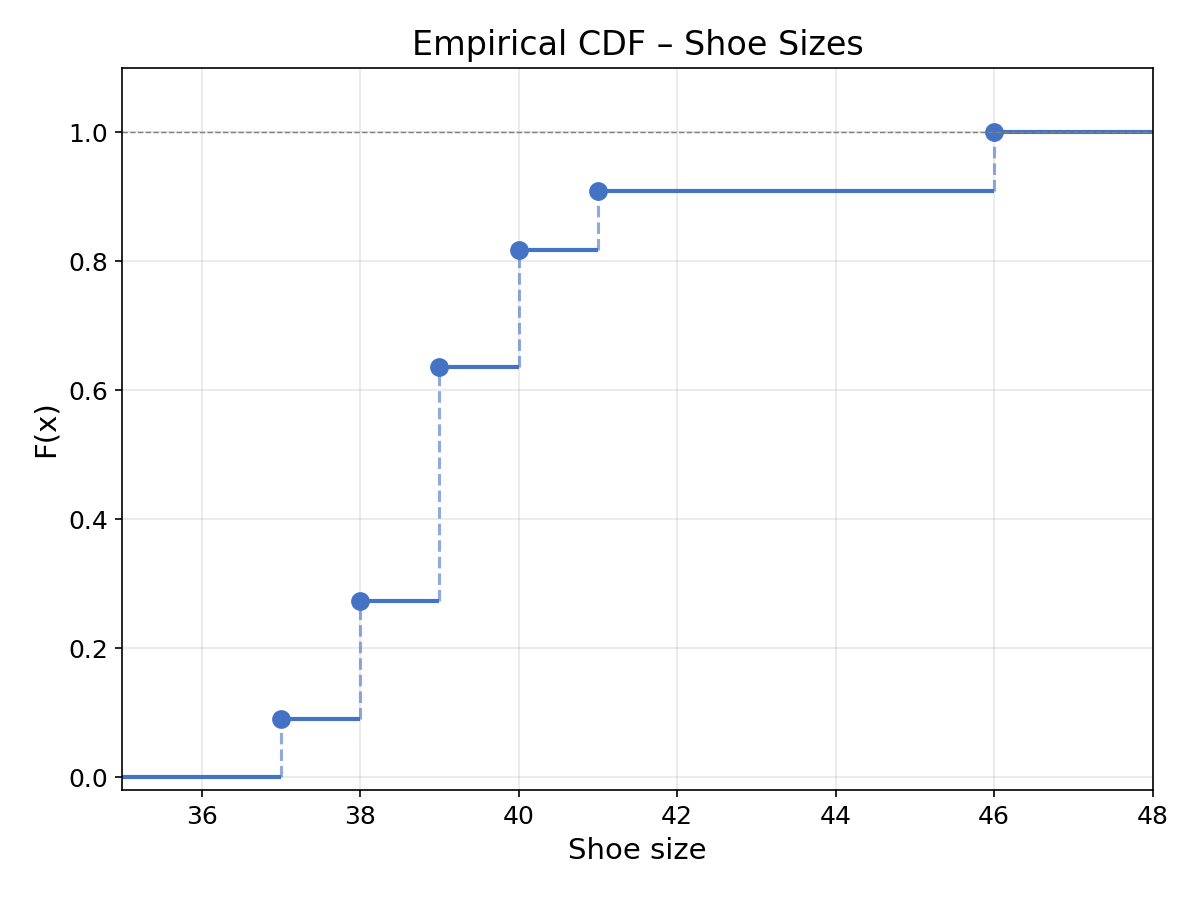
\includegraphics[width=0.8\textwidth,height=0.75\textheight,keepaspectratio]{images/image_004.png}
  \end{center}
\end{frame}

\begin{frame}{Empirical CDF -- Definition}
  \begin{block}{Definition}
    \[ F(x) = \sum_{x_i \leq x} f(x_i) \]
  \end{block}

  \vspace{0.3cm}

  \begin{itemize}
    \item Shows the cumulative proportion of the sorted values
    \item Computing the quantiles for every observed value yields the empirical CDF
    \item Quantiles can therefore be read off directly from it
  \end{itemize}
\end{frame}

\begin{frame}{Empirical CDF -- Reading Off Quantiles}
  \textbf{Example: Median.} The median is the smallest value at which the empirical CDF reaches $0.5$:
  \[ F(x_{0.5}) = 0.5 \quad \Leftrightarrow \quad F^{-1}(0.5) = x_{0.5} \]

  \vspace{0.3cm}

  \begin{block}{Generalisation}
    Every quantile ($0 \leq \alpha \leq 1$) can be obtained from the empirical CDF:
    \[ F(x_{\alpha}) = \alpha \quad \Leftrightarrow \quad F^{-1}(\alpha) = x_{\alpha} \]
  \end{block}
\end{frame}

% Slide 56: ECDF - Image
\begin{frame}{Empirical CDF}
  \begin{center}
    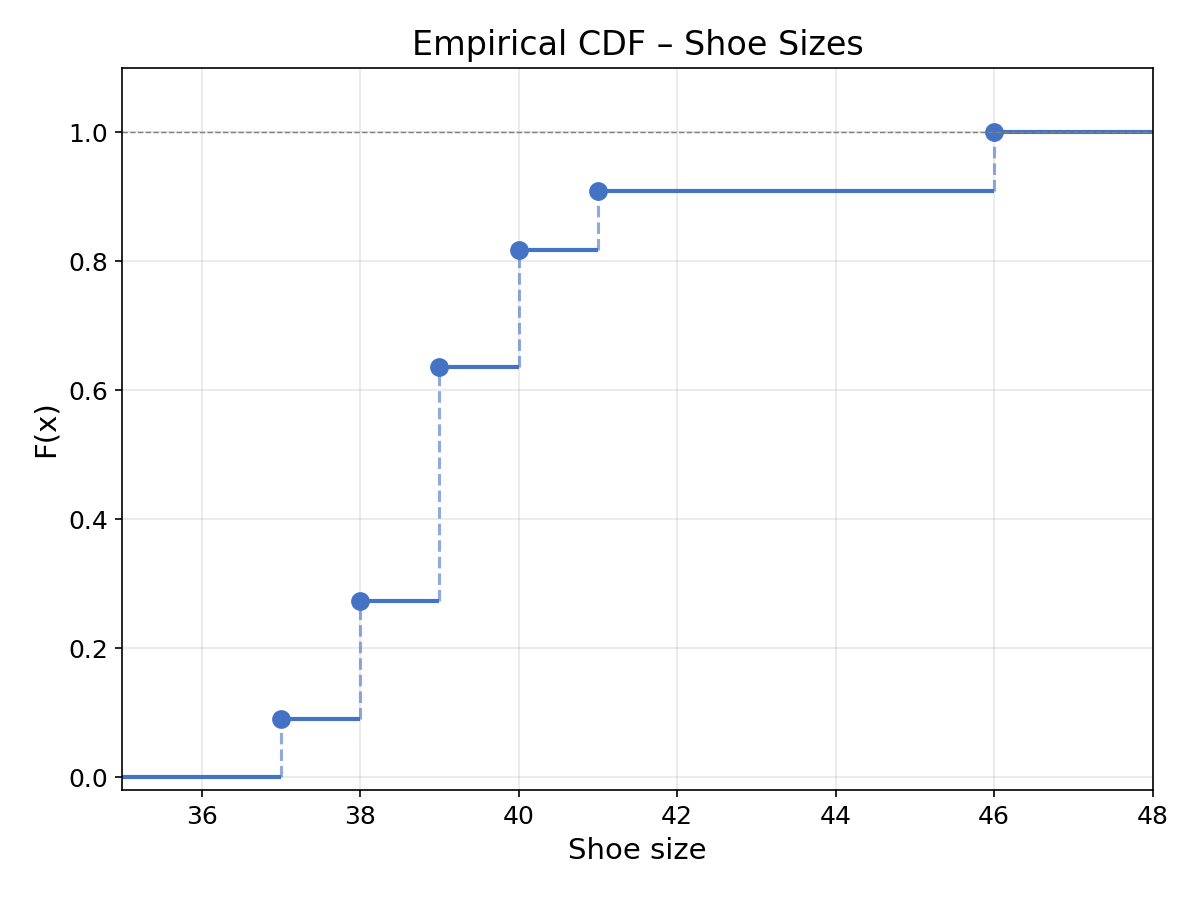
\includegraphics[width=0.8\textwidth,height=0.75\textheight,keepaspectratio]{images/image_004.png}
  \end{center}
\end{frame}

% Slide 57: ECDF in Python
\begin{frame}[fragile]{Empirical CDF in Python}
  \begin{block}{Computing}
    \begin{lstlisting}
import numpy as np, matplotlib.pyplot as plt
from statsmodels.distributions.empirical_distribution import ECDF
shoe = np.array([40, 39, 38, 41, 46, 39, 39, 38, 37, 40, 39])
F = ECDF(shoe)    # F is a function of x
    \end{lstlisting}
  \end{block}
  \begin{block}{Evaluating}
    \begin{lstlisting}
F(39)             # value of the empirical CDF at x = 39: 0.6364 (= 7/11)
    \end{lstlisting}
  \end{block}
  \begin{block}{Plotting}
    \begin{lstlisting}
plt.ecdf(shoe)    # step function incl. vertical jumps (matplotlib >= 3.8)
    \end{lstlisting}
  \end{block}
\end{frame}

\section{Histogram}
\begin{frame}{Histogram}
  \small
  The histogram is a special type of bar chart used to visualise the distribution of metric data. What makes it special is that the observed values are not displayed individually but are grouped into \textbf{classes (bins/intervals)}.

  \begin{block}{Density}
    For each class, the \textbf{relative frequency} is computed and divided by the class width:
    \[ \text{density} = \frac{\text{relative frequency of the class}}{\text{class width}} \]
    The bar height equals this density, so that the \textbf{area of each bar} represents the proportion of observations in the corresponding class.
  \end{block}

  \begin{itemize}
    \item Classes are defined by interval boundaries
    \item The choice of class width has a strong effect on the shape of the histogram
    \item Classes of different widths are also possible
  \end{itemize}
\end{frame}

% Slide 59: Histogram Example
\begin{frame}{Histogram -- Example}
  \begin{center}
    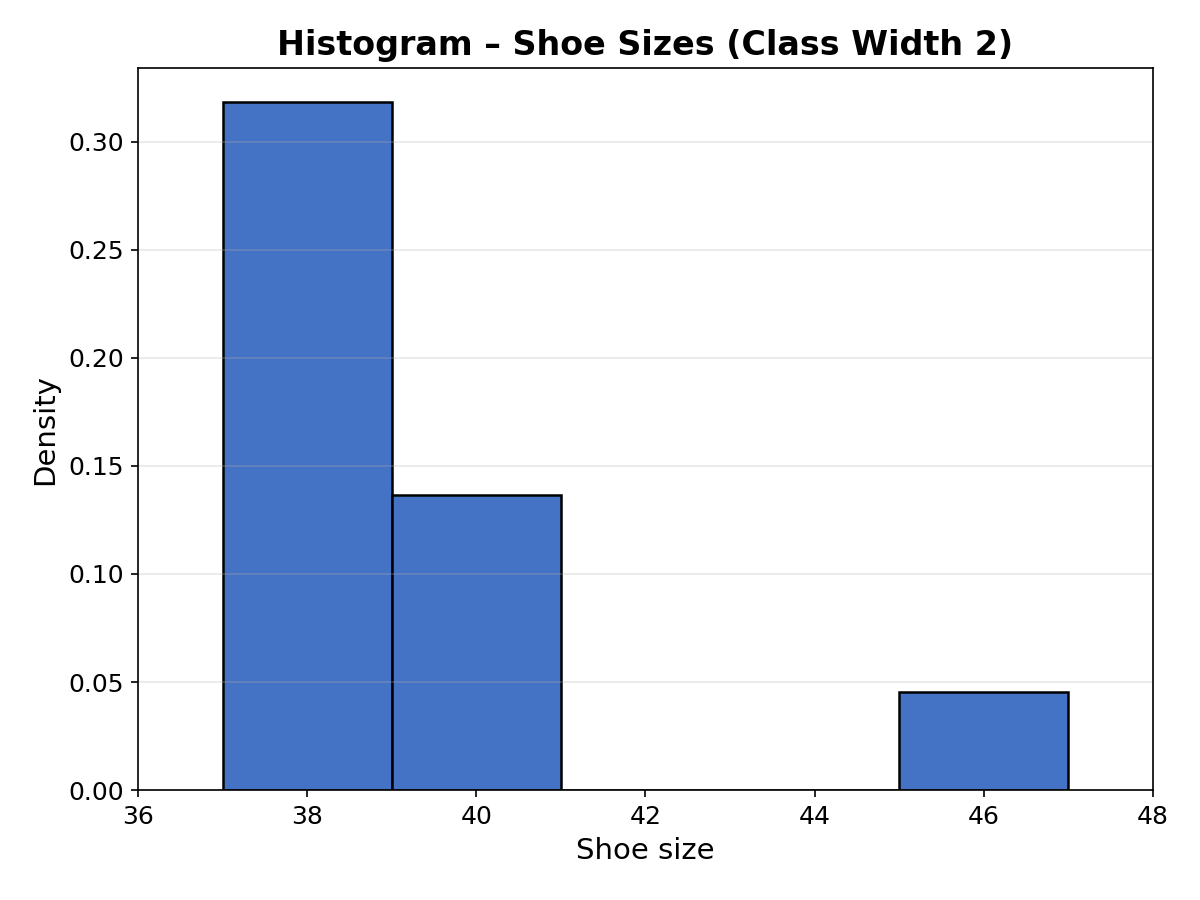
\includegraphics[width=0.8\textwidth,height=0.75\textheight,keepaspectratio]{images/hist_kb2.png}
  \end{center}
\end{frame}

\begin{frame}{Histogram -- Construction (Steps)}
  \begin{enumerate}
    \item \textbf{Define the classes}
      \begin{itemize}
        \item Notation: $[$ = inclusive, $($ = exclusive
          \begin{itemize}
            \item $[37,39]$: both 37 and 39 belong to the class
            \item $(39,41]$: 39 does \textbf{not} belong, 41 does
          \end{itemize}
        \item Each class is open on the left and closed on the right: $(a, b]$
        \item This way every value is assigned to \textbf{exactly one} class
        \item Exception: the \textbf{first} class is closed on both sides $[a, b]$ so that the smallest value is not lost
        \item e.\,g.\ $[37,39],\;(39,41],\;(41,43],\;(43,45],\;(45,47]$
      \end{itemize}
    \item \textbf{Count the observations in each class} $\to$ absolute frequencies
    \item \textbf{Compute the relative frequencies}
    \item \textbf{Divide the relative frequencies by the class width} $=$ density
    \item \textbf{Draw the bars} with heights equal to these densities
  \end{enumerate}
\end{frame}

\begin{frame}{Histogram -- Construction (Table)}
  Shoe sizes: 40, 39, 38, 41, 46, 39, 39, 38, 37, 40, 39 \quad ($n = 11$)

  \vspace{0.3cm}

  \begin{center}
    \small
    \begin{tabular}{lccccc@{\hspace{1.5em}}c}
      \toprule
      Class & $[37,39]$ & $(39,41]$ & $(41,43]$ & $(43,45]$ & $(45,47]$ & Total \\
      \midrule
      Class width & 2 & 2 & 2 & 2 & 2 & \\
      Abs.\ frequency & 7 & 3 & 0 & 0 & 1 & 11 \\
      Rel.\ frequency & $0.6364$ & $0.2727$ & $0$ & $0$ & $0.0909$ & $1$ \\[2pt]
      Density $= \frac{f_j}{\text{CW}}$ & $0.3182$ & $0.1364$ & $0$ & $0$ & $0.0455$ & \\
      \bottomrule
    \end{tabular}
  \end{center}

  \vspace{0.3cm}

  \begin{exampleblock}{Example: first class}
    Density $= \frac{0.6364}{2} = 0.3182$
  \end{exampleblock}
\end{frame}

% Slide 62: Histogram Example 2
\begin{frame}{Histogram -- Example}
  \begin{center}
    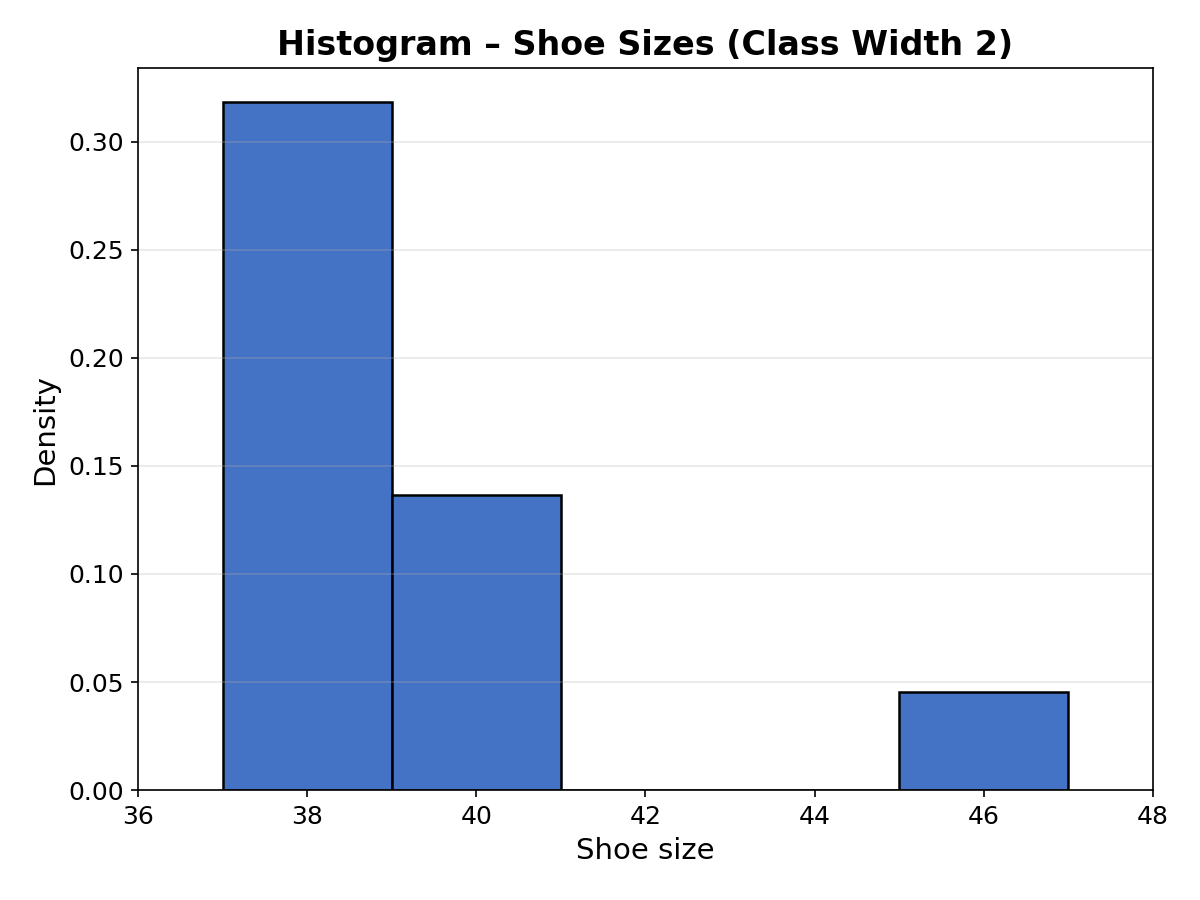
\includegraphics[width=0.8\textwidth,height=0.75\textheight,keepaspectratio]{images/hist_kb2.png}
  \end{center}
\end{frame}


\begin{frame}{Histogram -- Alternative Classes (Class Width 3)}
  Shoe sizes: 40, 39, 38, 41, 46, 39, 39, 38, 37, 40, 39 \quad ($n = 11$)

  \vspace{0.3cm}

  \begin{center}
    \small
    \begin{tabular}{lccc@{\hspace{1.5em}}c}
      \toprule
      Class & $[37,40]$ & $(40,43]$ & $(43,46]$ & Total \\
      \midrule
      Class width & 3 & 3 & 3 & \\
      Abs.\ frequency & 9 & 1 & 1 & 11 \\
      Rel.\ frequency & $0.8182$ & $0.0909$ & $0.0909$ & $1$ \\[2pt]
      Density $= \frac{f_j}{\text{CW}}$ & $0.2727$ & $0.0303$ & $0.0303$ & \\
      \bottomrule
    \end{tabular}
  \end{center}

  \vspace{0.3cm}

  \begin{exampleblock}{Example: first class}
    Density $= \frac{0.8182}{3} = 0.2727$
  \end{exampleblock}
\end{frame}

\begin{frame}{Histogram -- Unequal Class Widths}
  Shoe sizes: 40, 39, 38, 41, 46, 39, 39, 38, 37, 40, 39 \quad ($n = 11$)

  \vspace{0.3cm}

  \begin{center}
    \small
    \begin{tabular}{lcccc@{\hspace{1.5em}}c}
      \toprule
      Class & $[37,39]$ & $(39,40]$ & $(40,41]$ & $(41,46]$ & Total \\
      \midrule
      Class width & 2 & 1 & 1 & 5 & \\
      Abs.\ frequency & 7 & 2 & 1 & 1 & 11 \\
      Rel.\ frequency & $0.6364$ & $0.1818$ & $0.0909$ & $0.0909$ & $1$ \\[2pt]
      Density $= \frac{f_j}{\text{CW}}$ & $0.3182$ & $0.1818$ & $0.0909$ & $0.0182$ & \\
      \bottomrule
    \end{tabular}
  \end{center}

  \vspace{0.3cm}

  \begin{exampleblock}{Example: last class}
    Density $= \frac{0.0909}{5} = 0.0182$
 \end{exampleblock}
\end{frame}

\begin{frame}{Histogram -- Alternative Class Partition}
  \begin{center}
    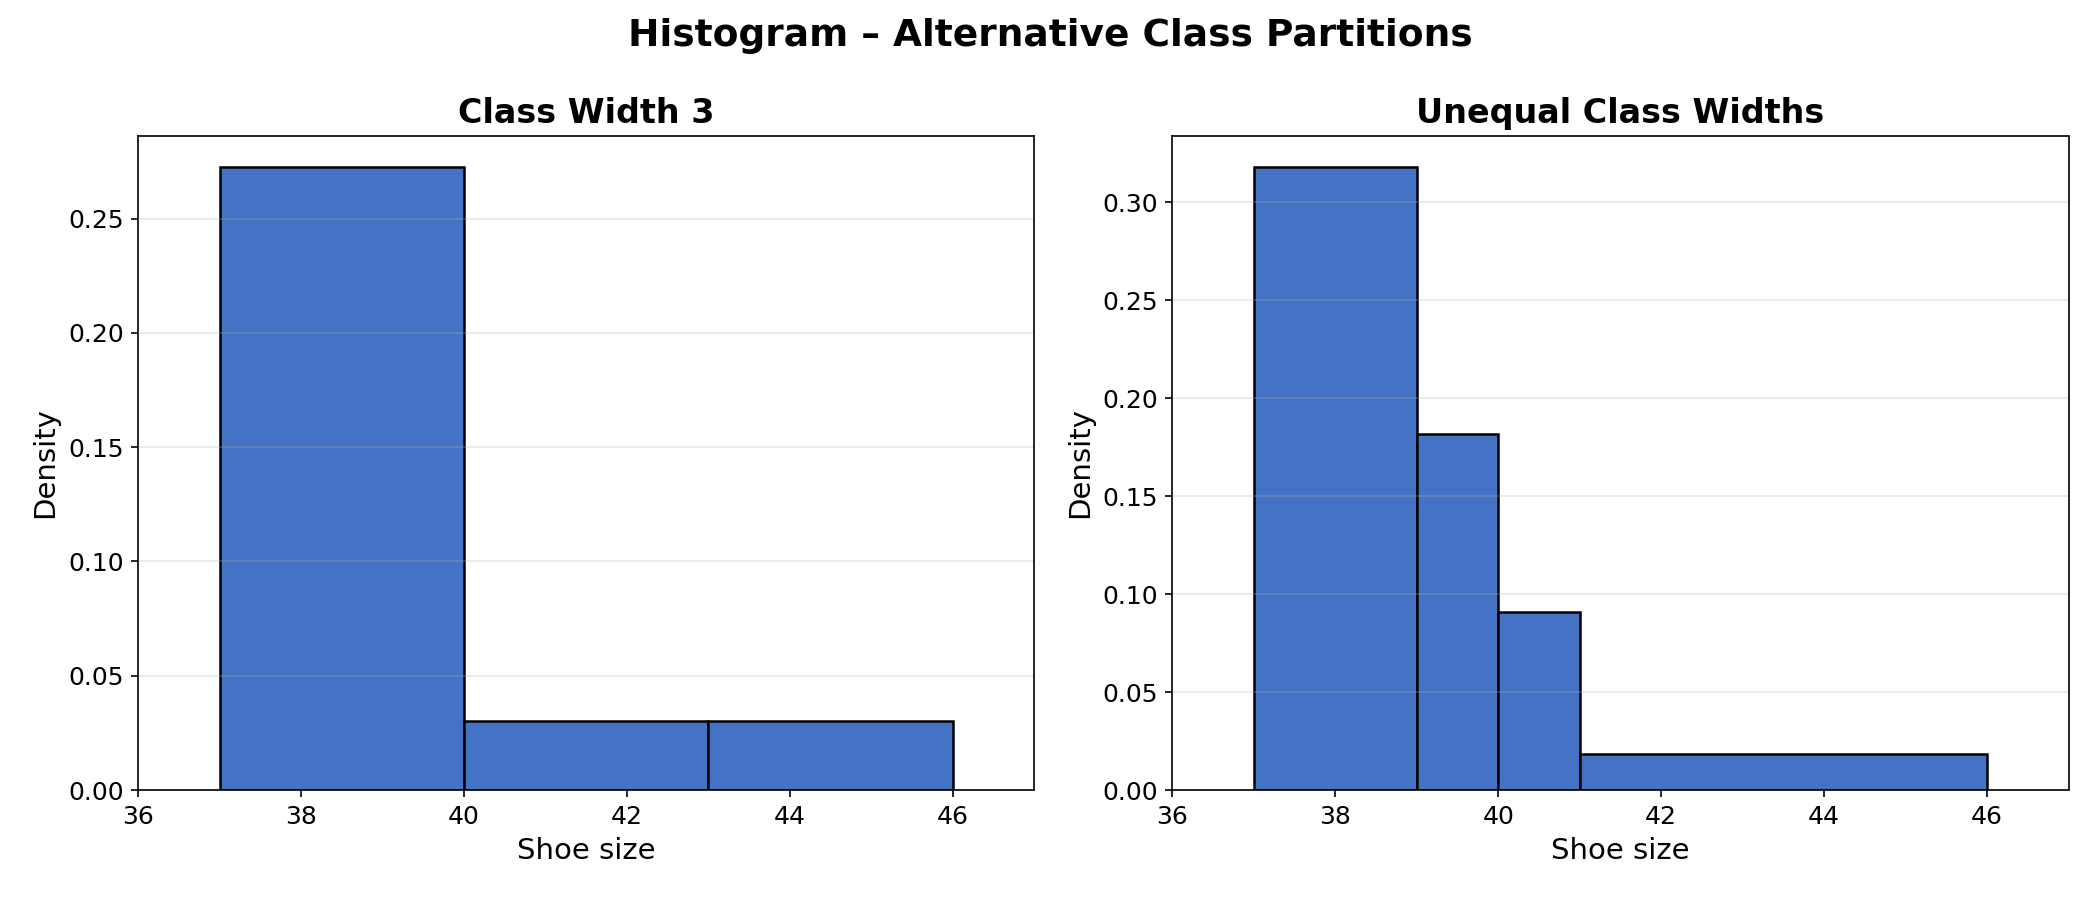
\includegraphics[width=\textwidth,height=0.78\textheight,keepaspectratio]{images/hist_andere_klassen.png}
  \end{center}
\end{frame}

\begin{frame}[fragile]{Histograms in Python}
  \begin{block}{Class width 2}
    \begin{lstlisting}
import pandas as pd
breaks = [37, 39, 41, 43, 45, 47]          # alternative: np.arange(37, 48, 2)
cls = pd.cut(shoe, breaks, right=True, include_lowest=True)  # [37,39], (39,41], ...
f = pd.Series(cls).value_counts(normalize=True, sort=False)   # rel. frequencies f_j
w = np.diff(breaks)                        # class widths
dens = f.to_numpy() / w                    # densities: 0.3182 0.1364 0 0 0.0455
plt.bar(breaks[:-1], dens, width=w, align="edge", edgecolor="black")
    \end{lstlisting}
  \end{block}

  \begin{block}{Unequal class widths}
    \begin{lstlisting}
breaks = [37, 39, 40, 41, 46]              # then the same lines as above   
                                           # densities: 0.3182 0.1818 0.0909 0.0182
    \end{lstlisting}
  \end{block}
  \footnotesize Why not simply \texttt{plt.hist}? It uses classes $[a,b)$ -- see
  \emph{Python Commands: Histogram}.
\end{frame}


% Slide 68: Exercise Histogram
\begin{frame}{Exercise -- Histogram}
  Create a histogram for the soccer team's shoe sizes using a class width of 2.
\end{frame}

% Slide 69: The Data
\begin{frame}{The Data}
  Shoe sizes: 40, 39, 38, 41, 46, 39, 39, 38, 37, 40, 39
\end{frame}

% Slide 70: Histogram Construction - Table
\begin{frame}{Histogram -- Construction (Table)}
  Shoe sizes: 40, 39, 38, 41, 46, 39, 39, 38, 37, 40, 39 \quad ($n = 11$)

  \vspace{0.3cm}

  \begin{center}
    \small
    \begin{tabular}{lccccc@{\hspace{1.5em}}c}
      \toprule
      Class & $[37,39]$ & $(39,41]$ & $(41,43]$ & $(43,45]$ & $(45,47]$ & Total \\
      \midrule
      Class width & 2 & 2 & 2 & 2 & 2 & \\
      Abs.\ frequency & 7 & 3 & 0 & 0 & 1 & 11 \\
      Rel.\ frequency & $0.6364$ & $0.2727$ & $0$ & $0$ & $0.0909$ & $1$ \\[2pt]
      Density $= \frac{f_j}{\text{CW}}$ & $0.3182$ & $0.1364$ & $0$ & $0$ & $0.0455$ & \\
      \bottomrule
    \end{tabular}
  \end{center}

  \vspace{0.3cm}

  \begin{exampleblock}{Example: first class}
    Density $= \frac{0.6364}{2} = 0.3182$
  \end{exampleblock}
\end{frame}

% Slide 71: Histogram Example
\begin{frame}{Histogram -- Example}
  \begin{center}
    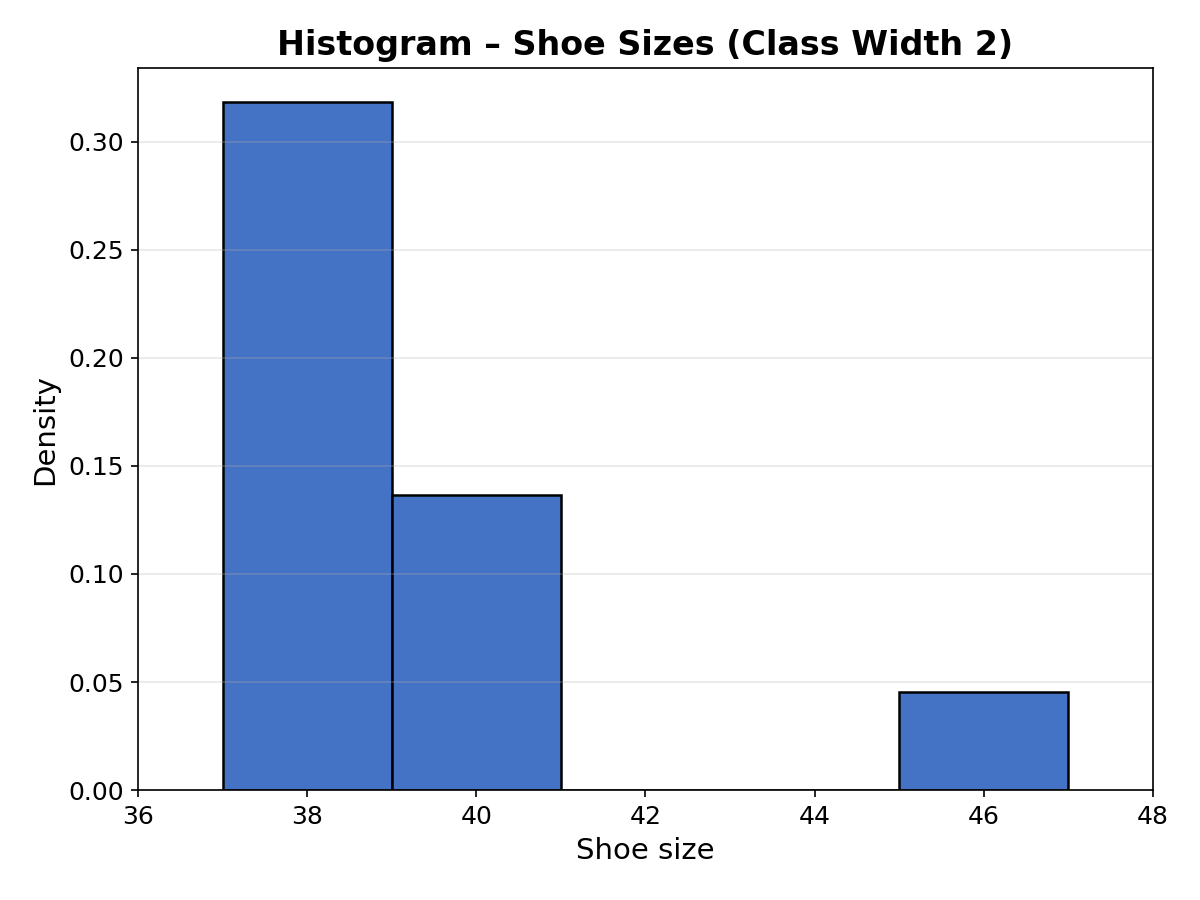
\includegraphics[width=0.8\textwidth,height=0.75\textheight,keepaspectratio]{images/hist_kb2.png}
  \end{center}
\end{frame}

\begin{frame}[fragile]{Python Commands: Histogram}
  \begin{alertblock}{Trap: \texttt{plt.hist} and \texttt{np.histogram} use classes $[a,b)$}
    Ours: $(a,b]$, first class $[a,b]$. NumPy: a boundary value goes to the class on its \textbf{right}.
    \begin{lstlisting}
np.histogram(shoe, bins=[37, 39, 41, 43, 45, 47], density=True)[0]
# [0.1364 0.2727 0.0455 0. 0.0455]   <- not our densities!
    \end{lstlisting}
  \end{alertblock}
  \begin{block}{Why?}
    $39$ (four times) and $41$ lie on class boundaries: $39$ falls into $[39,41)$ instead of
    $[37,39]$, $41$ into $[41,43)$ instead of $(39,41]$ -- \texttt{plt.hist} draws these wrong bars.
  \end{block}
  \begin{block}{Remedy}
    Classes with \texttt{pd.cut(..., right=True, include\_lowest=True)}, bars with \texttt{plt.bar} (next slide).
  \end{block}
\end{frame}

\begin{frame}[fragile]{Python Commands: Histogram with Our Classes}
  \begin{block}{Correct: classes with \texttt{pd.cut}, bars with \texttt{plt.bar}}
    \begin{lstlisting}
def density_hist(x, breaks):
    cls = pd.cut(x, breaks, right=True, include_lowest=True)
    f = pd.Series(cls).value_counts(normalize=True, sort=False)
    w = np.diff(breaks)                                  # class widths
    plt.bar(breaks[:-1], f / w, width=w, align="edge", edgecolor="black")
    return f / w                                         # densities f_j / w_j

density_hist(shoe, [37, 39, 41, 43, 45, 47])   # 0.3182 0.1364 0 0 0.0455
density_hist(shoe, [37, 39, 40, 41, 46])       # 0.3182 0.1818 0.0909 0.0182
    \end{lstlisting}
  \end{block}
  \begin{itemize}
    \item \texttt{right=True}: classes $(a,b]$; \texttt{include\_lowest=True}: first class closed $[a,b]$.
    \item Bar heights are the densities $f_j/\Delta x_j$, so every bar area equals $f_j$.
    \item The densities reproduce the tables of this section exactly.
  \end{itemize}
\end{frame}

\begin{frame}[fragile]{Python Commands: Classified Frequencies}
  \begin{block}{Class partition}
    \begin{lstlisting}
breaks = [37, 39, 41, 43, 45, 47]          # class boundaries b0, b1, ..., bk
cls = pd.cut(shoe, breaks, right=True, include_lowest=True)
    \end{lstlisting}
  \end{block}
  \begin{block}{Absolute classified frequencies}
    \begin{lstlisting}
pd.Series(cls).value_counts(sort=False)                   # 7 3 0 0 1
    \end{lstlisting}
  \end{block}
  \begin{block}{Relative classified frequencies}
    \begin{lstlisting}
pd.Series(cls).value_counts(normalize=True, sort=False)   # 0.6364 0.2727 0 0 0.0909
    \end{lstlisting}
  \end{block}
  \footnotesize pandas labels the first class \texttt{(36.999, 39.0]} -- this is
  exactly the closed class $[37,39]$.
\end{frame}

\section{Boxplot}
% Slide 72: Boxplot Definition
\begin{frame}{Boxplot}
  \begin{block}{Definition}
    A graphical display that highlights only the most important summary values of a dataset and thereby visualises the distribution of the data.
  \end{block}
\end{frame}

% Slide 73: Boxplot Image
\begin{frame}{Boxplot}
  \begin{center}
    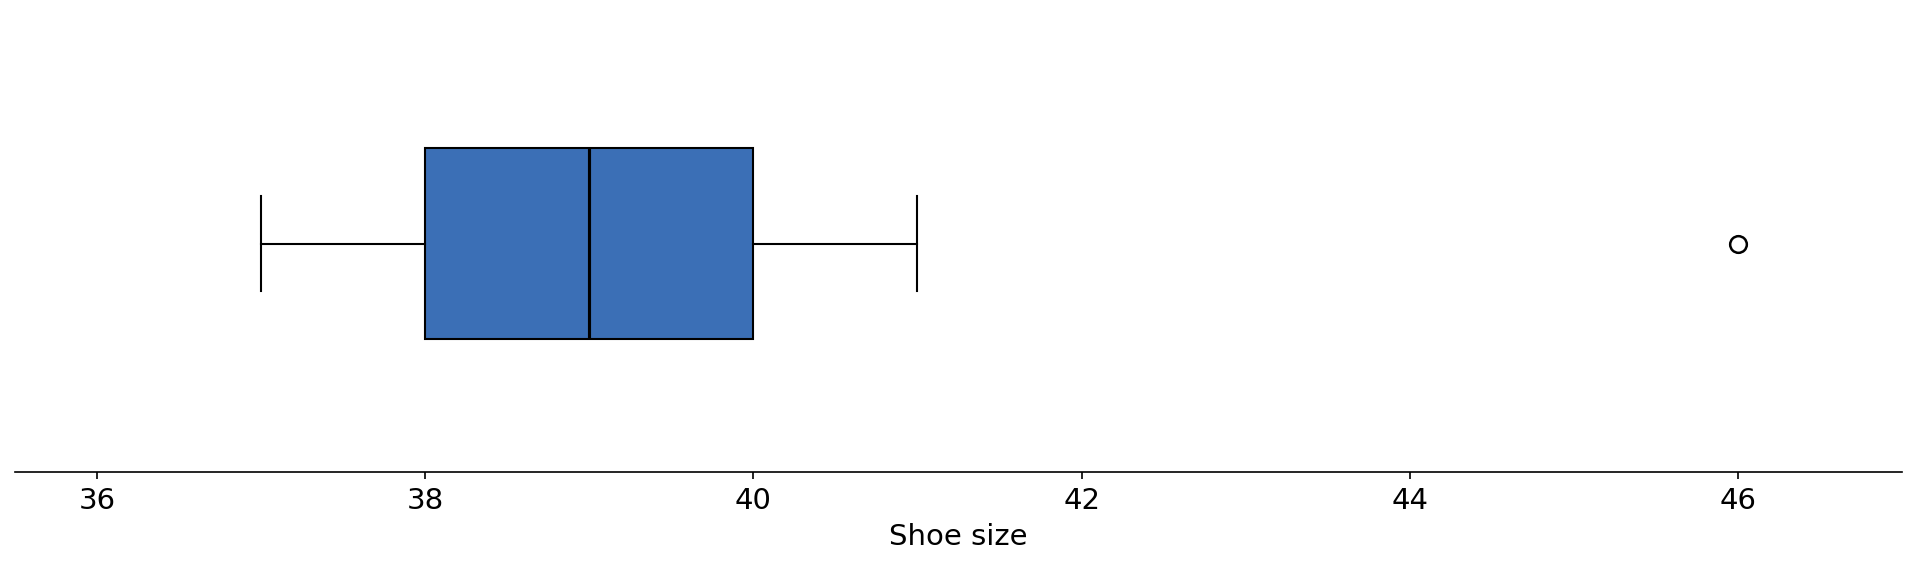
\includegraphics[width=\textwidth,height=0.75\textheight,keepaspectratio]{images/boxplot_schuhgroessen_clean.png}
  \end{center}
\end{frame}

% Slide 74 & 75: Boxplot with labels
\begin{frame}{Boxplot -- with Labels}
  \begin{center}
    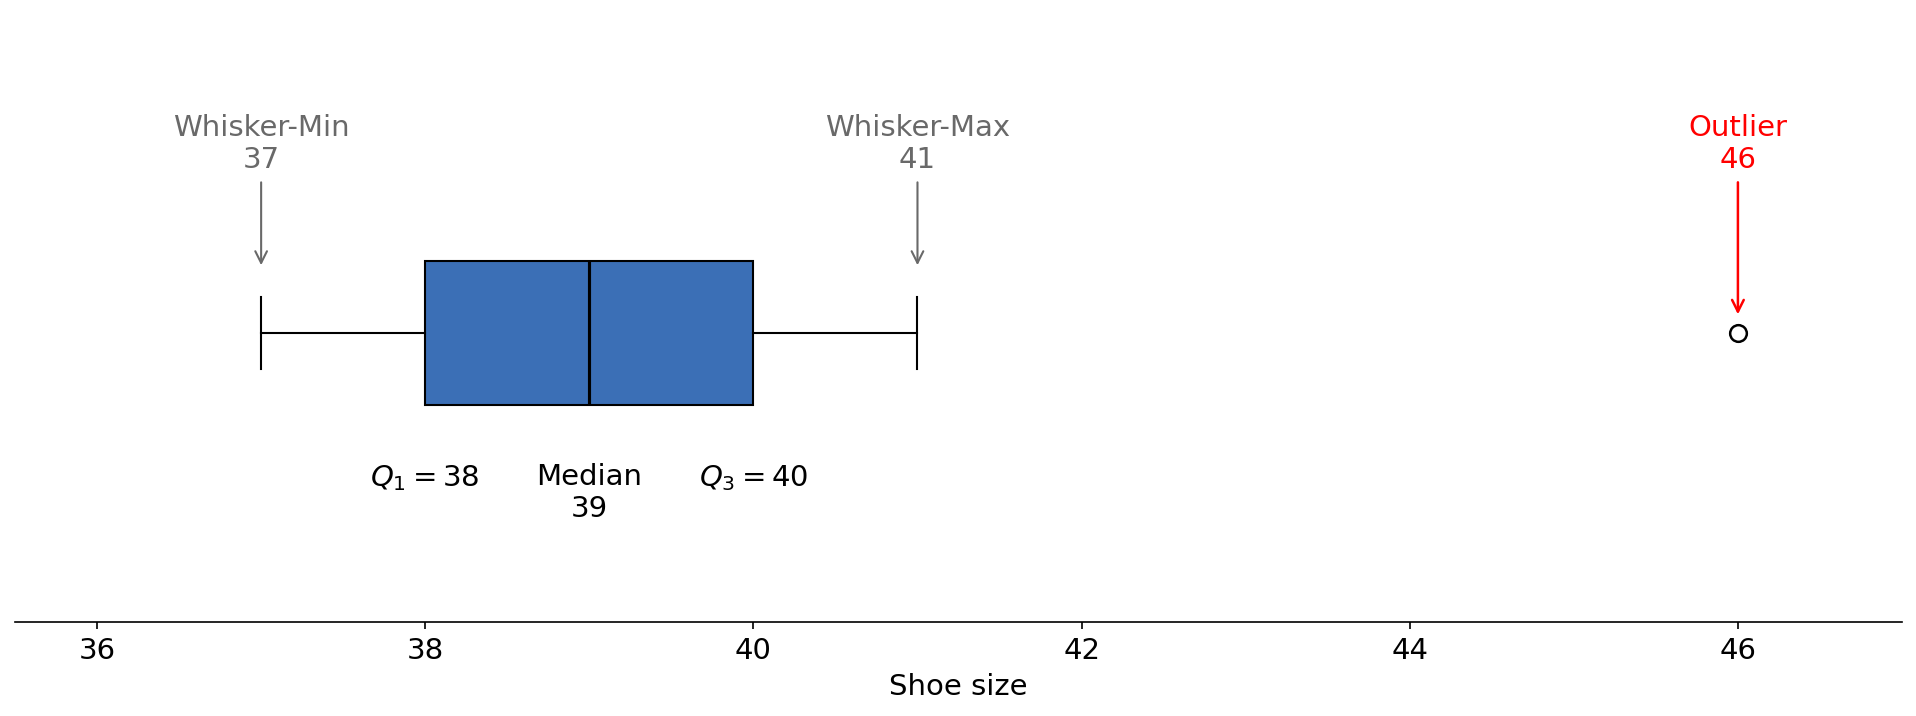
\includegraphics[width=\textwidth,height=0.75\textheight,keepaspectratio]{images/boxplot_schuhgroessen.png}
  \end{center}
\end{frame}

% Slide 76: Boxplot Construction
\begin{frame}{Boxplot -- Construction}
  \begin{enumerate}
    \item Sort the data
    \item Determine the median
    \item Determine the 1st quartile
    \item Determine the 3rd quartile
    \item Determine the lower whisker
    \item Determine the upper whisker
    \item Are there any outliers?
    \item Draw the boxplot
  \end{enumerate}
\end{frame}

% Slide 77: Boxplot Construction - Table
\begin{frame}{Boxplot -- Construction (Data)}
  \begin{center}
    \renewcommand{\arraystretch}{1.05}
    \small
    \begin{tabular}{rrrl}
      \toprule
      \textbf{Player} & \textbf{Shoe size} & \textbf{Sorted} & \\
      \midrule
      1 & 40 & 37 & Lower whisker \\
      2 & 39 & 38 & \\
      3 & 38 & 38 & 1st quartile \\
      4 & 41 & 39 & \\
      5 & 46 & 39 & \\
      6 & 39 & 39 & Median \\
      7 & 39 & 39 & \\
      8 & 38 & 40 & \\
      9 & 37 & 40 & 3rd quartile \\
      10 & 40 & 41 & Upper whisker \\
      11 & 39 & 46 & Outlier \\
      \midrule
      \textbf{Sum} & \textbf{436} & \textbf{436} & \\
      \bottomrule
    \end{tabular}
  \end{center}
\end{frame}

\begin{frame}{Boxplot -- Construction (Quartiles)}
  $n = 11$

  \vspace{0.5cm}

  \begin{columns}[T]
  \begin{column}{0.7\textwidth}
  \begin{center}
    \small\renewcommand{\arraystretch}{1.1}
    \begin{tabular}{lcccc}
      \toprule
      & $p$ & $n \cdot p$ & $\lceil n \cdot p \rceil$ = position & Value \\
      \midrule
      1st quartile & $0.25$ & $2.75$ & 3 & 38 \\
      2nd quartile (median) & $0.50$ & $5.50$ & 6 & 39 \\
      3rd quartile & $0.75$ & $8.25$ & 9 & 40 \\
      \bottomrule
    \end{tabular}
  \end{center}
  \end{column}
  \begin{column}{0.26\textwidth}
  \begin{center}
    \renewcommand{\arraystretch}{1.1}
    \begin{tabular}{lr}
      \toprule
      Lower whisker & 37 \\
      $Q_1$ & 38 \\
      Median & 39 \\
      $Q_3$ & 40 \\
      Upper whisker & 41 \\
      Outlier & 46 \\
      \bottomrule
    \end{tabular}
  \end{center}
  \end{column}
  \end{columns}
\end{frame}

% Slide 78: Lower Whisker Computation
\begin{frame}{Lower Whisker -- Computation}
  The lower whisker is the \textbf{smallest data point that is not yet an outlier}.
  To find it, compute a lower bound -- every value below it is classified as an outlier.
  \begin{align*}
    \text{Whisker}_{\min} &= \min\{x_i \mid x_i \ge x_{0.25} - k(x_{0.75} - x_{0.25})\} \\
    &\text{with } k = 1.5 \\
    &= \min\{x_i \mid x_i \ge 38 - 1.5(40 - 38)\} \\
    &= \min\{x_i \mid x_i \ge 38 - 3\} \\
    &= \min\{x_i \mid x_i \ge 35\} = 37
  \end{align*}
  Since $37$ is the smallest data value $\ge 35$, the lower whisker ends at $37$.
\end{frame}

% Slide 78b: Lower Whisker Step by Step
\begin{frame}{Lower Whisker -- Step by Step}
  \begin{enumerate}
    \item \textbf{Compute the IQR:} the interquartile range is the difference
      between the 3rd and 1st quartile: $\text{IQR} = x_{0.75} - x_{0.25} = 40 - 38 = 2$
    \item \textbf{Compute the lower bound:} subtract $1.5$ times the IQR from
      the 1st quartile: $38 - 1.5 \cdot 2 = 38 - 3 = 35$
    \item \textbf{Check the data:} every data point \textbf{below} $35$
      would be an outlier.
    \item \textbf{Determine the lower whisker:} the smallest data value still
      $\ge 35$ becomes the lower whisker. In our dataset this is $37$.
  \end{enumerate}
  \vspace{0.3cm}
  \begin{alertblock}{Interpretation}
    The lower whisker extends down to $37$ -- the smallest value that is not classified as an outlier.
    If a value $< 35$ existed, it would be shown separately as an outlier in the boxplot.
  \end{alertblock}
\end{frame}

% Slide 79: Upper Whisker Computation
\begin{frame}{Upper Whisker -- Computation}
  The upper whisker is the \textbf{largest data point that is not yet an outlier}.
  To find it, compute an upper bound -- every value above it is classified as an outlier.
  \begin{align*}
    \text{Whisker}_{\max} &= \max\{x_i \mid x_i \le x_{0.75} + k(x_{0.75} - x_{0.25})\} \\
    &\text{with } k = 1.5 \\
    &= \max\{x_i \mid x_i \le 40 + 1.5(40 - 38)\} \\
    &= \max\{x_i \mid x_i \le 43\} = 41
  \end{align*}
  Since $46 > 43$, the value $46$ is an outlier!
\end{frame}

% Slide 79b: Upper Whisker Step by Step
\begin{frame}{Upper Whisker -- Step by Step}
  \begin{enumerate}
    \item \textbf{Compute the IQR:} the interquartile range is the difference
      between the 3rd and 1st quartile: $\text{IQR} = x_{0.75} - x_{0.25} = 40 - 38 = 2$
    \item \textbf{Compute the upper bound:} add $1.5$ times the IQR to
      the 3rd quartile: $40 + 1.5 \cdot 2 = 40 + 3 = 43$
    \item \textbf{Check the data:} every data point \textbf{above} $43$
      would be an outlier.
    \item \textbf{Determine the upper whisker:} the largest data value still
      $\le 43$ becomes the upper whisker. In our dataset this is $41$.
  \end{enumerate}
  \vspace{0.3cm}
  \begin{alertblock}{Interpretation}
    The upper whisker extends up to $41$ -- the largest value that is not classified as an outlier.
    Since $46 > 43$, the value $46$ lies above the upper bound and is shown as a separate point in the boxplot.
  \end{alertblock}
\end{frame}

% Slide 80a: Boxplot Interpretation -- Symmetry and Median
\begin{frame}{Boxplot -- Interpretation (1/3): Symmetry and Median}
  \begin{block}{Symmetry}
    A boxplot is \textbf{symmetric} when the median lies in the centre of the box
    and both whiskers have the same length. This indicates that the data are
    evenly distributed around the centre.
  \end{block}
  \vspace{0.3cm}
  \begin{block}{Position of the median}
    The median splits the box into two halves. If it does \textbf{not} lie in the
    middle, the distribution is \textbf{skewed}:
    \begin{itemize}
      \item Median in the \textbf{left} half of the box $\rightarrow$
        \textbf{right-skewed} (positively skewed): many small values,
        a few large values pull the distribution to the right.
      \item Median in the \textbf{right} half of the box $\rightarrow$
        \textbf{left-skewed} (negatively skewed): many large values,
        a few small values pull the distribution to the left.
    \end{itemize}
  \end{block}
\end{frame}

% Slide 80b: Boxplot Interpretation -- Box and Whiskers
\begin{frame}{Boxplot -- Interpretation (2/3): Box and Whiskers}
  \begin{block}{Length of the box (IQR)}
    The box contains the middle $50\,\%$ of the data -- from the 1st quartile ($Q_1$)
    to the 3rd quartile ($Q_3$). A \textbf{wide box} indicates that these middle
    values are widely spread. A \textbf{narrow box} shows that half of the data
    lie close together.
  \end{block}
  \vspace{0.3cm}
  \begin{block}{Length of the whiskers}
    The whiskers extend from the box to the smallest and largest value that is
    not an outlier. If both whiskers are \textbf{equally long}, the distribution
    is symmetric in the tails.
    \textbf{Different whisker lengths} indicate that the data are more spread
    out in one direction than in the other.
  \end{block}
\end{frame}

% Slide 80c: Boxplot Interpretation -- Outliers and Example
\begin{frame}{Boxplot -- Interpretation (3/3): Outliers}
  \begin{block}{Outliers}
    Values that lie beyond the whiskers are shown individually as
    \textbf{outliers}. A value is considered an outlier if it lies more than
    $1.5$ times the IQR below $Q_1$ or above $Q_3$.
    Outliers can indicate measurement errors, special cases, or a strongly
    skewed distribution.
  \end{block}
  \vspace{0.3cm}
  \begin{exampleblock}{Example: shoe-size data}
    \begin{itemize}
      \item Box: $Q_1 = 38$, median $= 39$, $Q_3 = 40$ $\rightarrow$
        the median lies in the centre, the box is symmetric.
      \item Whiskers: min $= 37$, max $= 41$ $\rightarrow$
        both whiskers have the same length (each 1 unit from the box).
      \item Outlier: $46 > 43$ (upper bound) $\rightarrow$
        despite the symmetric box, the overall boxplot is \textbf{not} symmetric.
    \end{itemize}
  \end{exampleblock}
\end{frame}

% Slide 74 & 75: Boxplot with labels
\begin{frame}{Boxplot -- with Labels}
  \begin{center}
    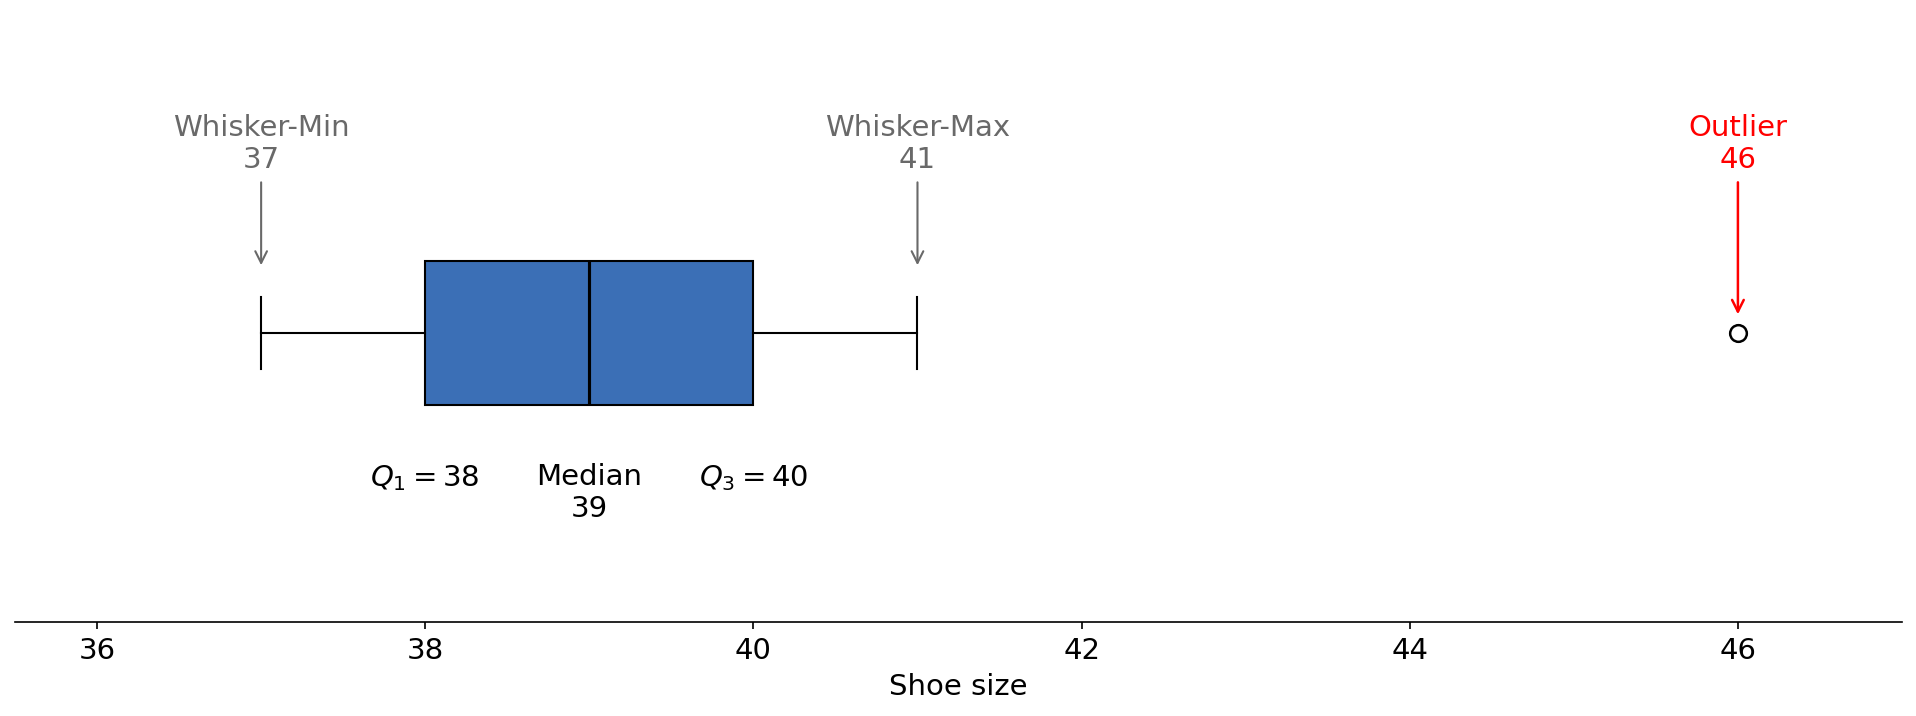
\includegraphics[width=\textwidth,height=0.75\textheight,keepaspectratio]{images/boxplot_schuhgroessen.png}
  \end{center}
\end{frame}


% Slide 84: Boxplot Conclusion
\begin{frame}{Boxplot -- Conclusion}
  \begin{block}{Advantages of the boxplot}
    \begin{itemize}
      \item Compact display of the \textbf{most important summary statistics}
        at a glance: median, quartiles, range and outliers.
      \item Allows a quick assessment of the \textbf{symmetry}
        and \textbf{skewness} of a distribution.
      \item Especially useful for \textbf{comparing several groups}
        side by side -- e.\,g.\ shoe sizes of different teams.
      \item \textbf{Outliers} are automatically detected
        and made visible.
    \end{itemize}
  \end{block}
  \vspace{0.3cm}
  \begin{alertblock}{Limitation}
    The boxplot reveals no information about the exact shape of the
    distribution inside the box -- two very different datasets can produce
    the same boxplot. To study the shape, a histogram is a useful complement.
  \end{alertblock}
\end{frame}

\section{Exercise}
\begin{frame}{Exercise: Body Heights -- Problem Statement}
  The body heights (in cm) of $n = 15$ persons are studied:
  \begin{center}
    164, 162, 168, 198, 166, 166, 192, 160, 151, 175, 180, 160, 168, 175, 168
  \end{center}
  \vspace{0.2cm}
  \textbf{Sorted:}
  \begin{center}
    151, 160, 160, 162, 164, 166, 166, 168, 168, 168, 175, 175, 180, 192, 198
  \end{center}
  \vspace{0.2cm}
  \begin{enumerate}
    \item Compute the mean, median, quartiles and the $17\,\%$ quantile.
    \item Compute the four measures of dispersion.
    \item Draw the empirical CDF, a histogram (class width $10$\,cm)
      and a boxplot.
    \item Draw the empirical CDF for the classified data (class midpoints).
  \end{enumerate}
\end{frame}

% Exercise
\begin{frame}{Exercise: Body Heights -- The Data}
  \begin{columns}[c]
  \begin{column}{0.66\textwidth}
  \centering
    \renewcommand{\arraystretch}{0.9}
    \footnotesize
    \begin{tabular}{cccccc}
      \toprule
      \textbf{Person} & \textbf{Height} & \textbf{Sorted} & \textbf{Abs.\ freq.} & \textbf{Rel.\ freq.} & \textbf{Cum.\ freq.} \\
      \midrule
      1  & 164 & 151 & 1 & $0.0\overline{6}$ & $0.0\overline{6}$ \\
      2  & 162 & 160 & 2 & $0.1\overline{3}$ & $0.2$ \\
      3  & 168 & 160 &   &   &   \\
      4  & 198 & 162 & 1 & $0.0\overline{6}$ & $0.2\overline{6}$ \\
      5  & 166 & 164 & 1 & $0.0\overline{6}$ & $0.3\overline{3}$ \\
      6  & 166 & 166 & 2 & $0.1\overline{3}$ & $0.4\overline{6}$ \\
      7  & 192 & 166 &   &   &   \\
      8  & 160 & 168 & 3 & $0.2$ & $0.\overline{6}$ \\
      9  & 151 & 168 &   &   &   \\
      10 & 175 & 168 &   &   &   \\
      11 & 180 & 175 & 2 & $0.1\overline{3}$ & $0.8$ \\
      12 & 160 & 175 &   &   &   \\
      13 & 168 & 180 & 1 & $0.0\overline{6}$ & $0.8\overline{6}$ \\
      14 & 175 & 192 & 1 & $0.0\overline{6}$ & $0.9\overline{3}$ \\
      15 & 168 & 198 & 1 & $0.0\overline{6}$ & $1$ \\
      \midrule
      \textbf{Sum} & \textbf{2553} & \textbf{2553} & \textbf{15} & \textbf{1} & \\
      \bottomrule
    \end{tabular}
  \end{column}
  \begin{column}{0.3\textwidth}
    \footnotesize
    \textbf{Note:} $\overline{6}$ denotes a repeating decimal, e.\,g.\
    \[ 0.0\overline{6} = 0.0666\ldots = \tfrac{1}{15} \]
  \end{column}
  \end{columns}
\end{frame}

% Results Overview
\begin{frame}{Exercise: Body Heights -- Results}
  \begin{center}
    \small
    \renewcommand{\arraystretch}{1.0}
    \begin{tabular}{lrr}
      \toprule
      \textbf{Statistic} & \textbf{Value} & \textbf{Bound} \\
      \midrule
      Sum                            & $2553$    & \\
      Arithmetic mean                & $170.2$ & \\
      Median                         & $168$     & \\
      Mode                           & $168$     & \\
      1st quartile                   & $162$     & \\
      3rd quartile                   & $175$     & \\
      $17\,\%$ quantile              & $160$     & \\
      Lower whisker                  & $151$     & $142.5$ \\
      Upper whisker                  & $192$     & $194.5$ \\
      \midrule
      Sample variance                & $151.60$ & \\
      Standard deviation             & $12.3126$  & \\
      Coefficient of variation       & $0.0723$   & \\
      Normalised coeff.\ of variation & $0.0187$   & \\
      \bottomrule
    \end{tabular}
  \end{center}
\end{frame}

% Step by Step: Mean
\begin{frame}{Exercise: Body Heights -- Mean (Step by Step)}
  \begin{block}{Formula}
    \[ \bar{x} = \frac{1}{n}\sum_{i=1}^{n} x_i \]
  \end{block}
  \vspace{0.2cm}
  \textbf{Step 1:} Sum all values:
  \begin{align*}
    \sum x_i &= 164 + 162 + 168 + 198 + 166 + 166 + 192 \\
             &\quad + 160 + 151 + 175 + 180 + 160 + 168 + 175 + 168 \\
             &= 2553
  \end{align*}
  \textbf{Step 2:} Divide by $n = 15$:
  \[
    \bar{x} = \frac{2553}{15} = 170.2\,\text{cm}
  \]
\end{frame}

% Step by Step: Median and Mode
\begin{frame}{Exercise: Body Heights -- Median and Mode}
  \textbf{Sorted data:}
  \begin{center}
    \small 151, 160, 160, 162, 164, 166, 166, \textbf{168}, 168, 168, 175, 175, 180, 192, 198
  \end{center}
  \vspace{0.2cm}
  \begin{block}{Median ($p = 0.5$)}
    $n \cdot p = 15 \cdot 0.5 = 7.5$ -- not an integer $\rightarrow$ round up to position $8$

    The 8th value in the sorted sequence is $\tilde{x}_{0.5} = \textbf{168}$\,cm.
  \end{block}
  \vspace{0.2cm}
  \begin{block}{Mode}
    The most frequent value: $168$ occurs $3$ times $\rightarrow \textbf{168}$\,cm.
  \end{block}
\end{frame}

% Step by Step: Quartiles and 17% quantile
\begin{frame}{Exercise: Body Heights -- Quartiles and Quantile}
  \textbf{Rule:} Compute $n \cdot p$. If the result is \textbf{not an integer},
  round up -- that position gives the desired value.
  \vspace{0.2cm}
  \begin{exampleblock}{$17\,\%$ quantile ($p = 0.17$)}
    $n \cdot p = 15 \cdot 0.17 = 2.55$ $\rightarrow$ round up to position $3$
    $\rightarrow x_{0.17} = 160$\,cm
  \end{exampleblock}
  \begin{exampleblock}{1st quartile ($p = 0.25$)}
    $n \cdot p = 15 \cdot 0.25 = 3.75$ $\rightarrow$ round up to position $4$
    $\rightarrow x_{0.25} = 162$\,cm
  \end{exampleblock}
  \begin{exampleblock}{3rd quartile ($p = 0.75$)}
    $n \cdot p = 15 \cdot 0.75 = 11.25$ $\rightarrow$ round up to position $12$
    $\rightarrow x_{0.75} = 175$\,cm
  \end{exampleblock}
\end{frame}

% Step by Step: Measures of Dispersion 1
\begin{frame}{Exercise: Body Heights -- Range and IQR}
  \begin{block}{Range}
    $R = x_{\max} - x_{\min} = 198 - 151 = \textbf{47}$\,cm
  \end{block}
  \vspace{0.3cm}
  \begin{block}{Interquartile range (IQR)}
    $\text{IQR} = x_{0.75} - x_{0.25} = 175 - 162 = \textbf{13}$\,cm
  \end{block}
  \vspace{0.3cm}
  The range reacts strongly to outliers (here: $198$),
  whereas the IQR is unaffected by them because it only considers the middle $50\,\%$ of the data.
\end{frame}

% Step by Step: Measures of Dispersion 2
\begin{frame}{Exercise: Body Heights -- Variance and Standard Deviation}
  \begin{block}{Sample variance}
    \[ s^2 = \frac{1}{n-1}\sum_{i=1}^{n}(x_i - \bar{x})^2 \]
  \end{block}
  \textbf{Step 1:} Square the deviations from the mean:
  \[
    (151 - 170.2)^2 = 368.64, \quad (160 - 170.2)^2 = 104.04, \quad \ldots
  \]
  \textbf{Step 2:} Sum of squared deviations:
  $\sum(x_i - \bar{x})^2 = 2122.40$

  \smallskip
  \textbf{Step 3:} Divide by $n - 1 = 14$:
  $s^2 = \dfrac{2122.40}{14} = \textbf{151.60}$\,cm$^2$

  \begin{block}{Standard deviation}
    $s = \sqrt{s^2} = \sqrt{151.60} = \textbf{12.3126}$\,cm
  \end{block}
\end{frame}

% Step by Step: Coefficient of variation
\begin{frame}{Exercise: Body Heights -- Coefficient of Variation}
  \begin{block}{Coefficient of variation}
    $v = \dfrac{s}{\bar{x}} = \dfrac{12.3126}{170.2} = \textbf{0.0723}$
  \end{block}
  \vspace{0.2cm}
  The coefficient of variation expresses the dispersion relative to the mean
  -- here the values scatter by about $7.2\,\%$ of the mean.
  \vspace{0.3cm}
  \begin{block}{Normalised coefficient of variation}
    $v^* = \dfrac{v}{\sqrt{n}} = \dfrac{0.0723}{\sqrt{15}} = \dfrac{0.0723}{3.8730} = \textbf{0.0187}$
  \end{block}
  \vspace{0.2cm}
  The normalised coefficient of variation additionally takes the sample size
  into account -- for larger $n$, $v^*$ becomes smaller because more
  observations stabilise the estimate of the mean.
\end{frame}

% Step by Step: Boxplot bounds
\begin{frame}{Exercise: Body Heights -- Whisker Computation}
  \begin{block}{Lower bound}
    $x_{0.25} - 1.5 \cdot \text{IQR} = 162 - 1.5 \cdot 13 = 162 - 19.5 = \textbf{142.5}$

    Smallest value $\ge 142.5$: lower whisker $= 151$
  \end{block}
  \vspace{0.2cm}
  \begin{block}{Upper bound}
    $x_{0.75} + 1.5 \cdot \text{IQR} = 175 + 1.5 \cdot 13 = 175 + 19.5 = \textbf{194.5}$

    Largest value $\le 194.5$: upper whisker $= 192$
  \end{block}
  \vspace{0.2cm}
  \begin{alertblock}{Outlier}
    $198 > 194.5$ $\rightarrow$ the value $198$ lies above the upper
    bound and is therefore an outlier.
  \end{alertblock}
\end{frame}



% Empirical CDF (task 3)
\begin{frame}{Exercise: Body Heights -- Empirical CDF}
  \begin{columns}[c]
    \begin{column}{0.64\textwidth}
      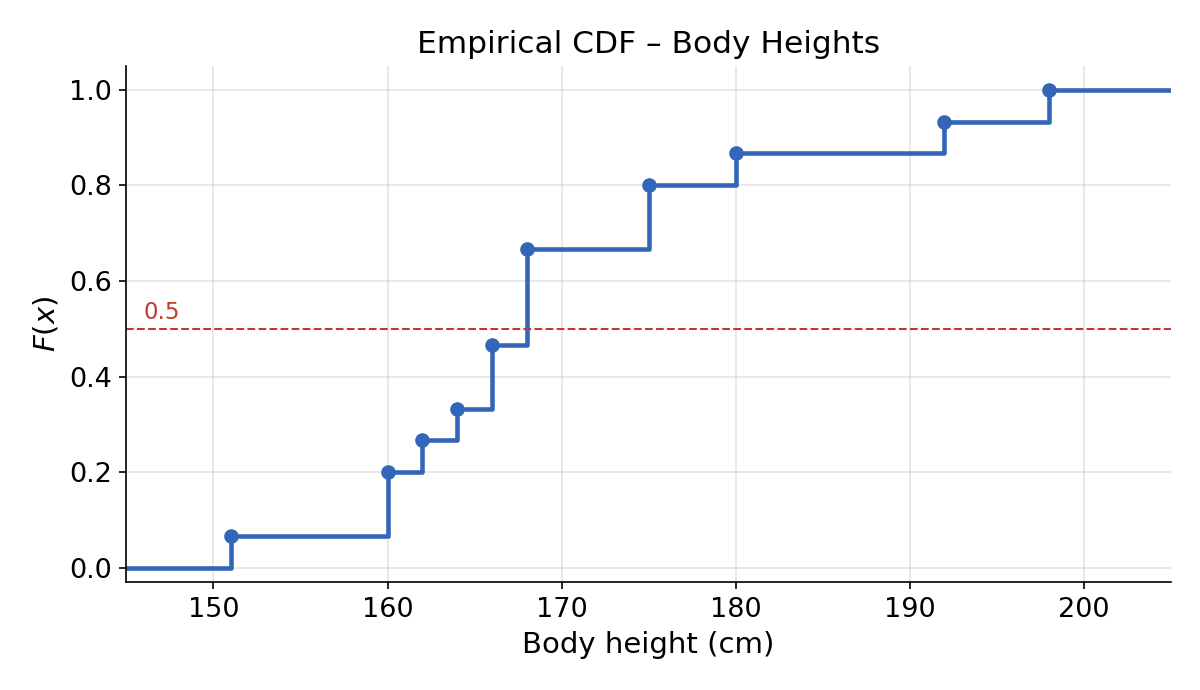
\includegraphics[width=\textwidth,height=0.72\textheight,keepaspectratio]{images/ecdf_body_heights.png}
    \end{column}
    \begin{column}{0.34\textwidth}
      \footnotesize
      \begin{itemize}\setlength{\itemsep}{4pt}
        \item Jump heights $=$ relative frequencies (e.\,g.\ $0.2$ at
              $168$\,cm, which occurs $3$ times).
        \item The step function first reaches $0.5$ at $x=168$
              $\Rightarrow$ median $\tilde{x}=168$\,cm.
        \item Values from the cumulative column of the data table.
      \end{itemize}
    \end{column}
  \end{columns}
\end{frame}

% Classified data (task 4)
\begin{frame}{Exercise: Body Heights -- Classified Data (Class Width 10\,cm)}
  \begin{center}
    \small
    \renewcommand{\arraystretch}{1.15}
    \begin{tabular}{lccccc@{\hspace{1.5em}}c}
      \toprule
      Class & $[150,160]$ & $(160,170]$ & $(170,180]$ & $(180,190]$ & $(190,200]$ & Total \\
      \midrule
      Class midpoint $a_j$ & $155$ & $165$ & $175$ & $185$ & $195$ & \\
      Abs.\ frequency $h_j$ & $3$ & $7$ & $3$ & $0$ & $2$ & $15$ \\
      Rel.\ frequency $f_j$ & $0.2$ & $0.4\overline{6}$ & $0.2$ & $0$ & $0.1\overline{3}$ & $1$ \\
      Cum.\ frequency $F(a_j)$ & $0.2$ & $0.\overline{6}$ & $0.8\overline{6}$ & $0.8\overline{6}$ & $1$ & \\
      \bottomrule
    \end{tabular}
  \end{center}
  \begin{exampleblock}{Construction}
    All observations of a class are placed at its \textbf{class midpoint}
    $a_j$; the empirical CDF then jumps by $f_j$ at each midpoint.
  \end{exampleblock}
\end{frame}

\begin{frame}{Exercise: Body Heights -- Empirical CDF of the Classified Data}
  \begin{columns}[c]
    \begin{column}{0.64\textwidth}
      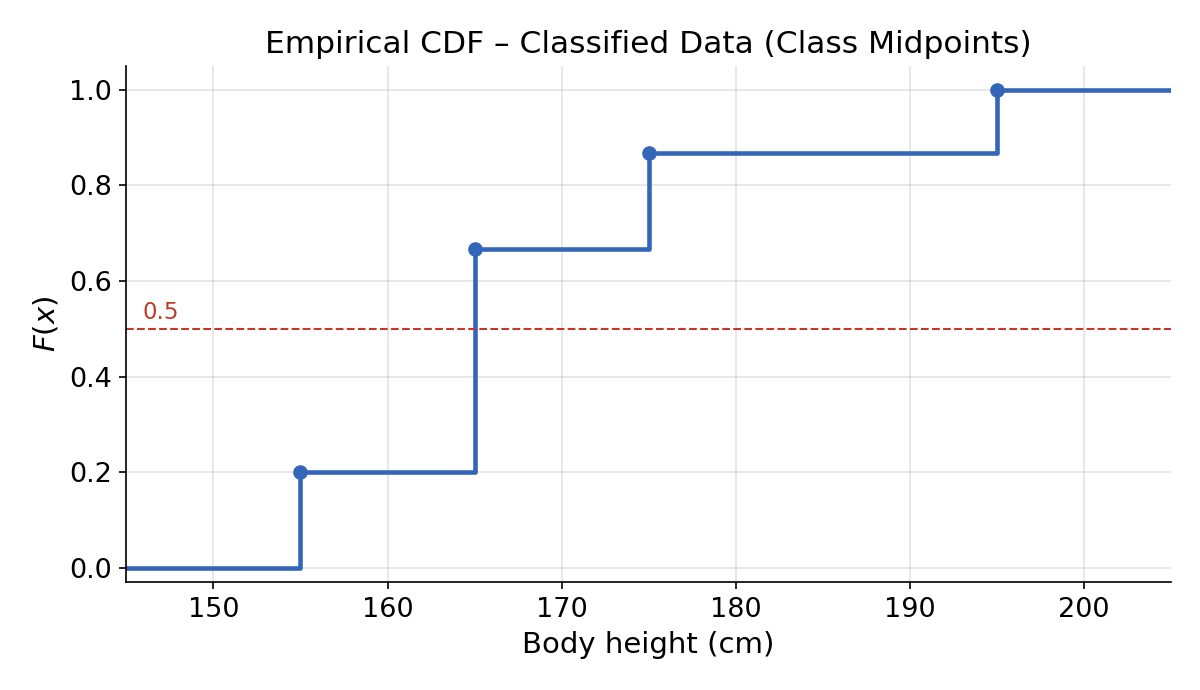
\includegraphics[width=\textwidth,height=0.72\textheight,keepaspectratio]{images/ecdf_body_heights_classified.png}
    \end{column}
    \begin{column}{0.34\textwidth}
      \footnotesize
      \begin{itemize}\setlength{\itemsep}{4pt}
        \item Only $4$ steps instead of $10$ -- the classified CDF is
              much \textbf{coarser}.
        \item It reaches $0.5$ at $a_2=165$, whereas the exact median is
              $168$\,cm.
      \end{itemize}
      \begin{alertblock}{Interpretation}
        Classifying the data simplifies the picture but \textbf{loses
        information}.
      \end{alertblock}
    \end{column}
  \end{columns}
\end{frame}

% Histogram
\begin{frame}{Exercise: Body Heights -- Histogram (Class Width 10\,cm)}
  \begin{center}
    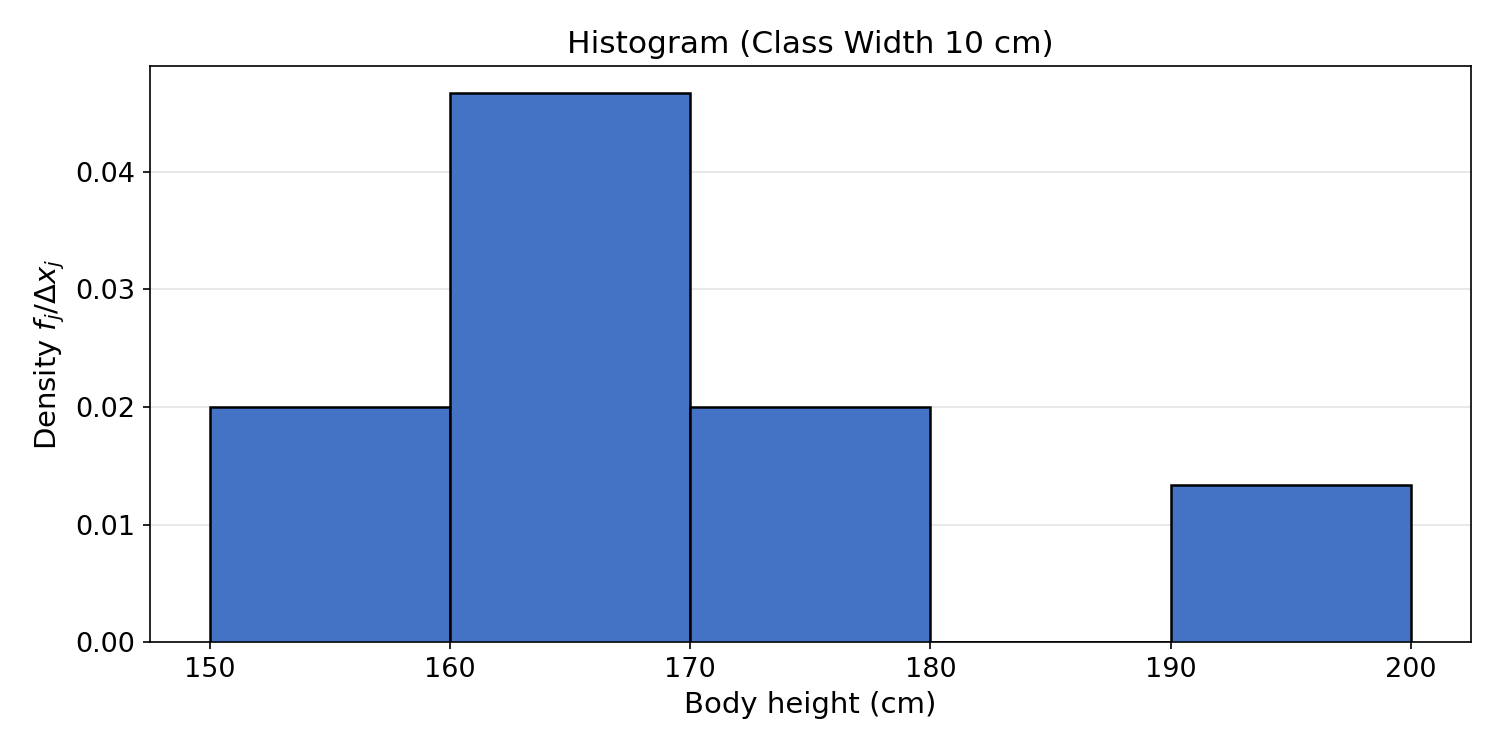
\includegraphics[width=0.95\textwidth,height=0.78\textheight,keepaspectratio]{images/hist_body_heights.png}
  \end{center}
\end{frame}

% Boxplot
\begin{frame}{Exercise: Body Heights -- Boxplot}
  \begin{center}
    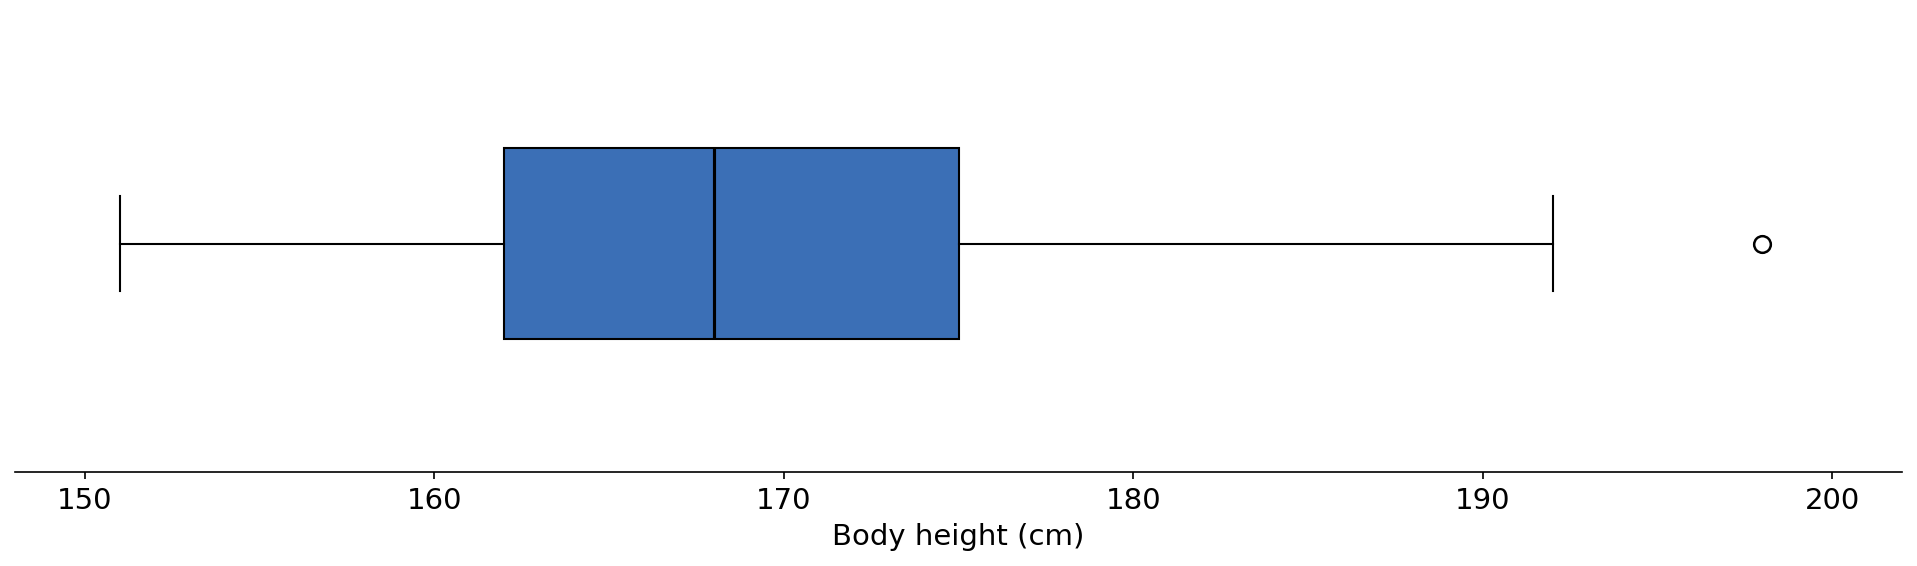
\includegraphics[width=0.95\textwidth,height=0.78\textheight,keepaspectratio]{images/boxplot_koerpergroesse.png}
  \end{center}
\end{frame}

\section[Python]{Python Commands}
% Python Commands: Frequencies and Measures of Central Tendency
\begin{frame}[fragile]{Python Commands: Frequencies and Measures of Central Tendency}
  \begin{block}{Absolute frequencies}
    \begin{lstlisting}
import numpy as np, pandas as pd
shoe = np.array([40, 39, 38, 41, 46, 39, 39, 38, 37, 40, 39])
tab = pd.Series(shoe).value_counts().sort_index()   # sorted by shoe size
print(tab)                                          # 37:1 38:2 39:4 40:2 41:1 46:1
    \end{lstlisting}
  \end{block}
  \begin{block}{Mean, median and quantiles}
    \begin{lstlisting}
np.mean(shoe)     # arithmetic mean: 39.6364
np.median(shoe)   # 39.0 -- note: averages for even n, not our definition!
# Better: method="inverted_cdf" matches our definition x_(ceil(n*p)):
np.quantile(shoe, 0.8, method="inverted_cdf")                # 80% quantile: 40
np.quantile(shoe, [0.25, 0.5, 0.75], method="inverted_cdf")  # quartiles: 38 39 40
    \end{lstlisting}
  \end{block}
\end{frame}

% Python Commands: Measures of Dispersion
\begin{frame}[fragile]{Python Commands: Measures of Dispersion}
  \begin{block}{Sample variance and standard deviation}
    \begin{lstlisting}
np.var(shoe, ddof=1)    # s^2 = 5.6545   (ddof=1: divide by n - 1)
np.std(shoe, ddof=1)    # s   = 2.3779
    \end{lstlisting}
  \end{block}
  \begin{block}{Coefficient of variation}
    \begin{lstlisting}
v = np.std(shoe, ddof=1) / np.mean(shoe)   # 0.0600
    \end{lstlisting}
  \end{block}
  \begin{block}{Normalised coefficient of variation}
    \begin{lstlisting}
vstar = v / np.sqrt(len(shoe))             # 0.0181
    \end{lstlisting}
  \end{block}
  \footnotesize Without \texttt{ddof=1}, NumPy divides by $n$ ($5.1405$ instead of
  $s^2 = 5.6545$); pandas' \texttt{.var()} and \texttt{.std()} already use \texttt{ddof=1}.
\end{frame}

% Python Commands: Empirical CDF
\begin{frame}[fragile]{Python Commands: Empirical CDF}
  \begin{block}{Computing and evaluating}
    \begin{lstlisting}
from statsmodels.distributions.empirical_distribution import ECDF
F = ECDF(shoe)
F(39)           # value of the ECDF at x = 39: 0.6364
    \end{lstlisting}
  \end{block}
  \begin{block}{Plotting}
    \begin{lstlisting}
import matplotlib.pyplot as plt
plt.ecdf(shoe)  # step function with vertical jumps
plt.show()
    \end{lstlisting}
  \end{block}
\end{frame}

% Python Commands: Histogram
\begin{frame}[fragile]{Python Commands: Histogram}
  \begin{block}{Equal class widths (here: 2)}
    \begin{lstlisting}
density_hist(shoe, [37, 39, 41, 43, 45, 47])   # 0.3182 0.1364 0 0 0.0455
density_hist(shoe, np.arange(37, 48, 2))       # same breaks, generated
    \end{lstlisting}
  \end{block}
  \begin{block}{Unequal class widths}
    \begin{lstlisting}
density_hist(shoe, [37, 39, 40, 41, 46])       # 0.3182 0.1818 0.0909 0.0182
    \end{lstlisting}
  \end{block}
  \footnotesize \texttt{density\_hist} (\texttt{pd.cut} + \texttt{plt.bar}) is defined in the
  Histogram section. Do \textbf{not} use \texttt{plt.hist(shoe, bins=breaks, density=True)}:
  its classes are $[a,b)$, so $39$ and $41$ would be counted in the wrong class.
\end{frame}

% Python Commands: Classified Frequencies
\begin{frame}[fragile]{Python Commands: Classified Frequencies}
  \begin{block}{Absolute frequencies}
    \begin{lstlisting}
pd.Series(shoe).value_counts().sort_index()
    \end{lstlisting}
  \end{block}
  \begin{block}{Class partition}
    \begin{lstlisting}
cls = pd.cut(shoe, bins=[37, 39, 41, 43, 45, 47], right=True, include_lowest=True)
    \end{lstlisting}
  \end{block}
  \begin{block}{Absolute and relative classified frequencies}
    \begin{lstlisting}
pd.Series(cls).value_counts(sort=False)                   # 7 3 0 0 1
pd.Series(cls).value_counts(normalize=True, sort=False)   # 0.6364 0.2727 0 0 0.0909
    \end{lstlisting}
  \end{block}
\end{frame}

% Python Commands: Boxplot
\begin{frame}[fragile]{Python Commands: Boxplot}
  \begin{block}{Standard boxplot (Tukey)}
    \begin{lstlisting}
plt.boxplot(shoe, vert=False, whis=1.5)   # horizontal, whiskers at k = 1.5
    \end{lstlisting}
    \texttt{whis} can be omitted for the default $k = 1.5$.
  \end{block}
  \begin{alertblock}{Trap: matplotlib interpolates the quartiles}
    \texttt{plt.boxplot} uses NumPy's default (linear interpolation), not our definition
    $x_{(\lceil n\cdot p\rceil)}$:
    \begin{lstlisting}
np.quantile(shoe, [0.25, 0.75])                          # [38.5 40.] interpolated
np.quantile(shoe, [0.25, 0.75], method="inverted_cdf")   # [38 40]    our definition
    \end{lstlisting}
    The box would start at $38.5$ instead of $Q_1 = 38$ -- next slide: boxplot with our quartiles.
  \end{alertblock}
\end{frame}

\begin{frame}[fragile]{Python Commands: Boxplot with Our Quartile Definition}
  \begin{block}{Quartiles, whisker bounds, whiskers and outliers}
    \begin{lstlisting}
q1, med, q3 = np.quantile(shoe, [0.25, 0.5, 0.75], method="inverted_cdf")  # 38 39 40
iqr = q3 - q1                                    # IQR = 2
lo, hi = q1 - 1.5 * iqr, q3 + 1.5 * iqr          # bounds: 35.0  43.0
inside = shoe[(shoe >= lo) & (shoe <= hi)]
whislo, whishi = inside.min(), inside.max()      # whiskers: 37  41
outliers = shoe[(shoe < lo) | (shoe > hi)]       # outlier: [46]
    \end{lstlisting}
  \end{block}
  \begin{block}{Drawing the boxplot from exactly these statistics}
    \begin{lstlisting}
stats = dict(q1=q1, med=med, q3=q3, whislo=whislo, whishi=whishi, fliers=outliers)
plt.gca().bxp([stats], vert=False)
plt.show()
    \end{lstlisting}
  \end{block}
\end{frame}

% ============================================================
% ===== SECTION: SUMMARY =====
% ============================================================
\section{Summary}

% Slide 1/5: Empirical CDF
\begin{frame}{Summary (1/3) -- Empirical CDF}
  \begin{block}{Definition}
    \[
      F(x) \;=\; \sum_{x_i \leq x} f(x_i)
      \qquad \text{with values in } [0,1]
    \]
  \end{block}
  \begin{block}{Reading off quantiles}
    \[
      F(x_{\alpha}) = \alpha
      \quad \Longleftrightarrow \quad
      F^{-1}(\alpha) = x_{\alpha},
      \qquad 0 \leq \alpha \leq 1
    \]
    Special case: $F^{-1}(0.5) = \tilde{x}$ (median).
  \end{block}
  \begin{itemize}
    \item Step function showing the cumulative relative frequency.
    \item Jump height at $x_i$ equals $f(x_i)$.
    \item Every quantile can be read off directly.
  \end{itemize}
\end{frame}

% Slide 2/5: Histogram
\begin{frame}{Summary (2/3) -- Histogram}
  \begin{block}{Density of a class}
    \[
      \text{density}_j \;=\; \frac{f_j}{\Delta x_j}
      \;=\; \frac{\text{rel.\ frequency of class } j}{\text{class width}}
    \]
  \end{block}
  \begin{block}{Area = relative frequency}
    \[
      \text{area}_j \;=\; \text{density}_j \cdot \Delta x_j \;=\; f_j,
      \qquad \sum_j f_j = 1
    \]
  \end{block}
  \begin{itemize}
    \item Suitable for metric, classified data.
    \item Classes: $[a_1,a_2],\,(a_2,a_3],\,\ldots,\,(a_{k-1},a_k]$ (first class closed on both sides).
    \item The choice of class width strongly affects the shape.
    \item Unequal class widths are also possible -- bar heights remain densities.
  \end{itemize}
\end{frame}

% Slide 3/5: Boxplot
\begin{frame}{Summary (3/3) -- Boxplot}
  \begin{block}{Five-number summary}
    \[
      x_{\min}\ \text{(or lower whisker)},\ x_{0.25},\ \tilde{x},\ x_{0.75},\ x_{\max}\ \text{(or upper whisker)}
    \]
    \[
      \text{IQR} \;=\; x_{0.75} - x_{0.25}
    \]
  \end{block}
  \begin{block}{Whisker bounds (Tukey, $k = 1.5$)}
    \begin{align*}
      \text{Whisker}_{\min} &\;=\; \min\!\bigl\{x_i \mid x_i \geq x_{0.25} - k \cdot \text{IQR}\bigr\} \\
      \text{Whisker}_{\max} &\;=\; \max\!\bigl\{x_i \mid x_i \leq x_{0.75} + k \cdot \text{IQR}\bigr\}
    \end{align*}
  \end{block}
  \begin{alertblock}{Outliers}
    All values $< x_{0.25} - 1.5 \cdot \text{IQR}$ or $> x_{0.75} + 1.5 \cdot \text{IQR}$
    are displayed individually as outliers.
  \end{alertblock}
\end{frame}


\begin{frame}{Outlook: Part 3 -- Statistical Inference}
  \begin{block}{What we have so far}
    Parts~1 and~2 \textbf{describe} the data at hand -- in numbers and in
    pictures.
  \end{block}
  \begin{block}{Next part}
    We treat the data as a \textbf{sample} and infer back to the
    \textbf{population}: confidence intervals and hypothesis tests. The
    mean $\bar x$ and the standard deviation $s$ of Part~1 become the
    building blocks of every interval and every test.
  \end{block}
  \kernaussage{From describing a sample to drawing conclusions about the
  population -- honestly reporting the uncertainty.}
\end{frame}

\end{document}

